
%%%%%%%%%%%%%%%%%%%%%%%%%%%%%%%%%%%%%%%%%%%%%%%%%%%%%%%% 
%% Stratégie d'asservissement de robot et de caméra   %%
%%                                                    %% 
%% Author: Luigi Franco Tedesco                       %%
%%%%%%%%%%%%%%%%%%%%%%%%%%%%%%%%%%%%%%%%%%%%%%%%%%%%%%%% 

% \documentclass[twocolumn,notitlepage,11pt]{report}
% \documentclass[a4paper,notitlepage,11pt]{report}
% \documentclass[a4paper,notitlepage,twoside,10pt]{report}
% \documentclass[a4paper,notitlepage,twoside,11pt]{report}
\documentclass{report}

\usepackage[english,french]{babel}
\usepackage[utf8]{inputenc}
% \usepackage{lmodern}
% \usepackage{textcomp}% symboles supplémentaires
\usepackage{rotating}

\usepackage{amsmath}
\usepackage{gensymb}
\usepackage{amsfonts}
\usepackage{latexsym}
\usepackage{tabularx, lipsum}
\usepackage{amssymb}
\usepackage{probsoln}
\usepackage{enumerate}
\usepackage{tikz}
\usepackage{amssymb}
\usepackage{amsthm}
\usepackage{amsmath}
\usepackage{fancyhdr}
\usepackage{multirow}
\usepackage{stmaryrd}
\usepackage{listings}
\usepackage{color}
\usepackage{url}
\usepackage{bm}
\usepackage{soul}
\usepackage{palatino}
\usepackage{algorithm}
\usepackage{seqsplit}
\usepackage{pstricks}
\usepackage{framed}
\usepackage{array}
% \usepackage{gnuplottex}
\usepackage[miktex]{gnuplottex}
\usepackage{subfig}
\usepackage[noend]{algpseudocode}
\newtheorem{theorem}{Théorème}
\newtheorem{lemma}{Lemme}
\newtheorem{remark}{Remarque}
\newtheorem{definition}{Définition}
\newtheorem{property}{Propriété}
\newtheorem{problem}{Problème}


%\newenvironment{rappel}%
%{%
%\begin{framed}\textbf{Rappel:}%
%}
%{%
%\end{framed}%
%}%

\newsavebox{\fmbox}
\newenvironment{rappel}
{\begin{center}\begin{lrbox}{\fmbox}\begin{minipage}{0.7\textwidth}\textbf{Rappel :}}
{{\vskip 1mm \vskip 0cm}\end{minipage}\end{lrbox}\fbox{\usebox{\fmbox}}\end{center}}

\newenvironment{algo}[1]
{\begin{center}\begin{lrbox}{\fmbox}\begin{minipage}{0.9\textwidth}\textbf{#1 :}}
{{\vskip 1mm \vskip 0cm}\end{minipage}\end{lrbox}\fbox{\usebox{\fmbox}}\end{center}}


%\newenvironment{algo}[1]
%{\begin{minipage}{0.9\textwidth}\textbf{#1 :}}
%{\end{minipage}\\}
%\newenvironment{rappel}{\begin{center}
%\fbox{
%\begin{minipage}{0.7\textwidth}
%	\textbf{Rappel:}}
%{\end{minipage}
%}
%\end{center}}
%   before}{  after}
%\newenvironment{proof}[1][Proof]{\begin{trivlist}
%\item[\hskip \labelsep {\bfseries #1}]}{\end{trivlist}}
%\newenvironment{definition}[1][Definition]{\begin{trivlist}
%\item[\hskip \labelsep {\bfseries #1}]}{\end{trivlist}}
%\newenvironment{example}[1][Example]{\begin{trivlist}
%\item[\hskip \labelsep {\bfseries #1}]}{\end{trivlist}}
%\newenvironment{remark}[1][Remark]{\begin{trivlist}
%\item[\hskip \labelsep {\bfseries #1}]}{\end{trivlist}}

%\newcommand{\qed}{\nobreak \ifvmode \relax \else
%      \ifdim\lastskip<1.5em \hskip-\lastskip
%      \hskip1.5em plus0em minus0.5em \fi \nobreak
%      \vrule height0.75em width0.5em depth0.25em\fi}

\newcommand{\Mgrinv}[2]{\ensuremath{\mathbb{#1}/#2\mathbb{#1}^*}}
\newcommand{\Mgr}[2]{\ensuremath{\mathbb{#1}/#2\mathbb{#1}}}
\newcommand{\benolah}[1]{\ensuremath{\llbracket#1\rrbracket}}

\newcommand{\PC}[2]{\emph{#1}[\ensuremath{#2}]}

\newcommand{\HRule}{\rule{\linewidth}{0.5mm}}

\DeclareMathOperator{\pgcd}{pgcd}
\DeclareMathOperator{\ppmc}{ppmc}

\floatname{algorithm}{Algorithme}

\definecolor{gray}{gray}{0.3}
\definecolor{blue}{rgb}{0,0,0.5}
\definecolor{green}{rgb}{0,0.5,0}
\definecolor{lightgreen}{rgb}{0,0.6,0}
\definecolor{purple}{rgb}{0.5,0,0.5}
\definecolor{darkred}{rgb}{0.5,0,0}
\definecolor{dkgreen}{rgb}{0,0.6,0}
\definecolor{mauve}{rgb}{0.58,0,0.82}
\definecolor{orange}{rgb}{1,0.5,0}

\renewcommand{\lstlistingname}{Code}

\newcommand{\TODO}[1]{ \textcolor{red}{\large TODO:} \textcolor{purple}{[#1]~}}
\lstset{ %
  language=python,                % the language of the code
  basicstyle=\footnotesize\ttfamily,           % the size of the fonts that are used for the code
  numbers=left,                   % where to put the line-numbers
  numberstyle=\tiny\color{gray},  % the style that is used for the line-numbers
  stepnumber=1,                   % the step between two line-numbers. If it's 1, each line 
                                  % will be numbered
  numbersep=5pt,                  % how far the line-numbers are from the code
  backgroundcolor=\color{white},      % choose the background color. You must add \usepackage{color}
  showspaces=false,               % show spaces adding particular underscores
  showstringspaces=false,         % underline spaces within strings
  showtabs=false,                 % show tabs within strings adding particular underscores
  frame=single,                   % adds a frame around the code
  rulecolor=\color{black},        % if not set, the frame-color may be changed on line-breaks within not-black text (e.g. commens (green here))
  tabsize=2,                      % sets default tabsize to 2 spaces
  captionpos=b,                   % sets the caption-position to bottom
  breaklines=true,                % sets automatic line breaking
  breakatwhitespace=false,        % sets if automatic breaks should only happen at whitespace
  title=\lstname,                   % show the filename of files included with \lstinputlisting;
                                  % also try caption instead of title
%
	emph={access,and,as,break,class,continue,def,del,elif,else,%
	except,exec,finally,for,from,global,if,import,in,is,%
	lambda,not,or,pass,print,raise,return,try,while,assert},
	emphstyle=\color{orange}\bfseries,
	emph={[2]self},
	emphstyle=[2]\color{blue},
	emph={[4]ArithmeticError,AssertionError,AttributeError,BaseException,%
	DeprecationWarning,EOFError,Ellipsis,EnvironmentError,Exception,%
	False,FloatingPointError,FutureWarning,GeneratorExit,IOError,%
	ImportError,ImportWarning,IndentationError,IndexError,KeyError,%
	KeyboardInterrupt,LookupError,MemoryError,NameError,None,%
	NotImplemented,NotImplementedError,OSError,OverflowError,%
	PendingDeprecationWarning,ReferenceError,RuntimeError,RuntimeWarning,%
	StandardError,StopIteration,SyntaxError,SyntaxWarning,SystemError,%
	SystemExit,TabError,True,TypeError,UnboundLocalError,UnicodeDecodeError,%
	UnicodeEncodeError,UnicodeError,UnicodeTranslateError,UnicodeWarning,%
	UserWarning,ValueError,Warning,ZeroDivisionError,abs,all,any,apply,%
	basestring,bool,buffer,callable,chr,classmethod,cmp,coerce,compile,%
	complex,copyright,credits,delattr,dict,dir,divmod,enumerate,eval,%
	execfile,exit,file,filter,float,frozenset,getattr,globals,hasattr,%
	hash,help,hex,id,input,int,intern,isinstance,issubclass,iter,len,%
	license,list,locals,long,map,max,min,object,oct,open,ord,pow,property,%
	quit,range,raw_input,reduce,reload,repr,reversed,round,set,setattr,%
	slice,sorted,staticmethod,str,sum,super,tuple,type,unichr,unicode,%
	vars,xrange,zip},
	emphstyle=[4]\color{purple}\bfseries,					  
%
%
  keywordstyle=\color{blue},          % keyword style
  commentstyle=\color{dkgreen},       % comment style
  stringstyle=\color{mauve},         % string literal style
  escapeinside={\%*}{*)},            % if you want to add a comment within your code
  morekeywords={self,*,...}               % if you want to add more keywords to the set
}

\usepackage{hyperref}
\usepackage{enumitem}
\usepackage{etoolbox}

\usetikzlibrary{positioning}

\newtoggle{rapport}
\toggletrue{rapport}

%\usepackage[a4paper, left=3cm, right=2cm, top=2.5cm, bottom=2.5cm]{geometry}
\usepackage[a4paper,total={6in,9in}]{geometry}

\iftoggle{rapport}{ } {

} 



%%%% BEGIN DOCUMENT
\begin{document}

\pagenumbering{Roman}
\begin{titlepage}

	\begin{center}
	
		% Upper part of the page
		%
\includegraphics[width=0.26\textwidth]{enstalogo.png}\\[1cm]   
		% Logos
		\begin{minipage}{0.45\textwidth}
		\begin{flushleft}
			
\includegraphics[width=100px]{enstalogo.png}
		\end{flushleft}
		\end{minipage}
		\begin{minipage}{0.45\textwidth}
		\begin{flushright}
			
\includegraphics[width=100px]{upmclogo.png}
		\end{flushright}
		\end{minipage}
		\mbox{}\\[1.5cm] 

		\textbf{ \textsc{\Large Université Pierre et Marie Curie}\\[0.5cm] }
		
		\textbf{ \textsc{\Large École Nationale Supérieure de Techniques Avancées}\\[0.5cm]}
		
		\vfill
	
		\textsc{\large Projet de Fin d'Études}\\[0.5cm]
	
		% Title
	        %\hrule width \hsize \kern 1mm \hrule width \hsize height 2pt
		\HRule \\[0.4cm]
		{ \huge \bfseries Stratégie d'asservissement de robot et de caméra}\\[0.15cm]
	
	              %\hrule width \hsize \kern 1mm \hrule width \hsize height 2pt
		      \HRule \\[1.5cm]
	                
		% Author and supervisor
		\begin{minipage}{0.4\textwidth}
			\begin{flushleft} \large
				\textbf{Auteur}\\
				Luigi \textsc{Franco Tedesco}\\
				      \textit{tedesco@ensta.fr}\\
				Promotion 2015
			\end{flushleft}
		\end{minipage}
		\begin{minipage}{0.55\textwidth}
			\begin{flushright} \large
				\textbf{Professeurs Responsables} \\
				David \textsc{Filliat} \\
				\textit{david.filliat@ensta.fr}\\[0.1cm]
				Safia \textsc{Kedad-Sidhoum} \\
				\textit{Safia.Kedad-Sidhoum@lip6.fr}\\[0.1cm]
				\textbf{Tuteur} \\
				Jean-François \textsc{Goudou} \\
				\textit{jean-francois.goudou@thalesgroup.com}\\
			\end{flushright}
		\end{minipage}

		\vfill

		%{\color{red} Rapport {\bf non confidentiel} et {\bf publiable} sur internet}\\[0.2cm]
		\begin{tabular}{r|l}
			\multirow{2}{*}{THALES Service}& Campus Theresis\\
			       & 828 Boulevard des Maréchaux, 91762 Palaiseau 
		\end{tabular}\\[1cm]
		% Bottom of the page
		Stage éffectué du 09 mai 2015 au 28 août 2015\\[0.2cm]
		%{\large 28 août 2015}
		%{\large \today}
	\end{center}

\end{titlepage}



\newpage
\mbox{}
\thispagestyle{empty}

\newpage




% %\begin{abstract}\centering % Colocar somente 4 linhas aqui depois....
% il s'agit d'étudier un système de chiffrement à clef
%publique inventé par Pascal Paillier en 1999. Un premier volet du
%travail consistera en une revue des propriétés des anneaux modulaires
%nécessaires à la compréhension du mécanisme de
%chiffrement/déchiffrement. Ensuite il s'agira de comprendre sur quels
%problèmes calculatoirement difficiles repose ce cryptosystème. Des
%notions de théorie de la complexité pourront être appréhendées à cette
%occasion. Une troisième partie sera dédiée à la mise en oeuvre
%informatique de ce système cryptographique. Pour cela,
%l'étudiant utilisera une bibliothèque de manipulation de grands
%entiers. Les performances du système seront alors évaluées. 
%Le stage s'ouvrira ensuite vers une direction plus large qui est
%l'investigation des systèmes de chiffrement ayant des propriétés
%homomorphiques, dont le système de Paillier fait partie, et
%l'application de ce type de fonctionnalité à la résolution de 
%problématiques de la vie courante (ex. calcul sur des serveurs
%distants, vote électronique). 
%Dans ce cadre, des variantes du système de Paillier seront considérées.
%\end{abstract}
\vspace*{\stretch{1}}
\thispagestyle{empty}
\selectlanguage{french}%
\begin{abstract}\centering
\noindent Dans ce projet il a été étudié le système de chiffrement à clé
publique inventé par Pascal Paillier en 1999. Ici sont discutées les principales
caractéristiques du point de vue mathématique et cryptographique qui 
régissent le système. 
Ensuite il est exposé une analyse du système 
étendu proposé par Ivan Damgård et Mads Jurik. Les deux cryptosystèmes
ont été implantés en \verb!Python! et un test de performance a été fait pour 
mesurer empiriquement leur fonctionnement.

\end{abstract}

{\bf Mots-clés:} Cryptographie à Cle Publique, Système de Paillier  , Système de Damgard-Jurik, Résiduosité, Chiffrement Homomorphe.
%Paillier, Damgård-Jurik, Homomorphisme, clé publique, ré\-si\-duo\-sité.
\selectlanguage{english}%
\begin{abstract}\centering
\noindent This project aims at the study of the public key cryptosystem 
invented by Pascal Paillier in 1999. On this report both the
mathematical and cryptographic characteristics relatives to the
system will be discussed 
and an analysis of the extended system proposed by Ivan Damgård and Mads Jurik
will be conducted.
Both systems were implemented in \verb!Python! and a benchmark was realized 
in order to empirically evaluate both systems and their optimizations.
\end{abstract}

{\bf Keywords:} Public Key Cryptography     , Paillier Cryptosystem, Damgard-Jurik           , Residuosity, Homomorphic Encryption.
%Paillier, Damgård-Jurik, Homomorphic, public key, re\-si\-duo\-si\-ty.
\selectlanguage{french}%
\vspace*{\stretch{1}}

%%
%Cryptographie à Cle Publique, Système de Paillier  , Système de Damgard-Jurik, Résiduosité, Chiffrement Homomorphe.
%Public Key Cryptography     , Paillier Cryptosystem, Damgard-Jurik           , Residuosity, Homomorphic Encryption.

% \newpage
\mbox{}
\thispagestyle{empty}

\newpage




% \thispagestyle{empty}
\vspace*{\fill}
{\large{\center {\textbf{Remerciements}}\\[0.2cm]}

	\begin{minipage}[c]{\textwidth}
	\center
       Je remercie énormément Celine Craye pour son engagement et aide constant pendent tout le déroulement de mon stage. \\ Merci.
      \end{minipage}
}
\vspace*{\fill}
\newpage


% \newpage
\mbox{}
\thispagestyle{empty}

\newpage




% \thispagestyle{empty}
\vspace*{\fill}
{\center {\textbf{Attestation de non confidentialité}}\\[0.2cm]

	\begin{minipage}[c]{\textwidth}
	\center
	Par la présente, je soussignée Madame \textsc{Levy-dit-Vehel} Françoise, employée en tant que Enseignant-Chercheur dans l'\textbf{ENSTA Paristech} située au \textit{828, Boulevard des Maréchaux, 91762 Palaiseau Cedex}, atteste sur l'honneur que les données contenues dans le rapport de Monsieur \textsc{Pacianotto Gouveia} Gustavo \textbf{ne sont pas confidentielles}. Par conséquent, le contenu peut être communiqué et diffusé à l'extérieur sous format papier et/ou électronique.

      	\end{minipage}
}\\[3cm]

\begin{minipage}{0.95\textwidth}
\hfill à Palaiseau, le 13/09/2012.
\end{minipage}\\[1cm]
	\begin{minipage}{1.1\textwidth}
		\noindent\begin{minipage}{0.45\textwidth}
			\begin{flushleft} 

				{\center \rule{5cm}{1pt}	}\\
				\textbf{Élève}\\
				Gustavo \textsc{Pacianotto Gouveia}\\

				
			\end{flushleft}
		\end{minipage}
		\begin{minipage}{0.45\textwidth}
			\begin{flushright} 

				{\center \rule{5cm}{1pt}	}\\
				\textbf{Professeur Responsable} \\
				Françoise \textsc{Levy-dit-Vehel} \\


			\end{flushright}
		\end{minipage}
	\end{minipage}


\vspace*{\fill}
\newpage


%% Header and footer config
\pagestyle{fancy}
\fancyhead{}
\fancyfoot{}
%\addtolength{\headheight}{\baselineskip}
%\renewcommand{\sectionmark}[1]{\markboth{#1}{}}
%\renewcommand{\subsectionmark}[1]{\markright{#1}}
%\rhead{\leftmark\\\rightmark}
\renewcommand{\chaptermark}[1]{% 
\markboth{\thechapter.\ #1}{}} 
\renewcommand{\sectionmark}[1]{\markright{\thesection\ #1}}
\fancyhead[LE,RO]{\slshape {\normalsize \rightmark}}
\fancyhead[LO,RE]{\slshape {\normalsize  Méthode de reconnaissance d'objets multi-vues sur un robot mobile}}
\fancyfoot[C]{Luigi Franco \textbf{Tedesco} - THALES Service - Campus Theresis \\{\color{red}Rapport non confidentiel et publiable sur internet}}
\fancyfoot[RO,LE]{\thepage}
\renewcommand{\footrulewidth}{0.4pt}

\pagenumbering{arabic}
\setcounter{page}{4}
\tableofcontents

%%%% Introduction



\iftoggle{rapport} {
 \chapter{Introduction}
}
\textbf{La perception de l'environment par machines est indispensable pour son integration à la vie quotidienne. Compétences telle comme se localiser, prise de décisions et capacité d'apprentissage sont nécessaire pour la réalisation de les plus simples tâches. Dans cet étude, on s'intéresse à la compréhension d'éléments constituent d'une scène, sujet récurrent dans le domaine de la vision par ordinateur. Plusieurs approches proposés dans la littérature explorent une sous-partie du pipiline de la réconnaissance pour faire face au difficile défi de représenter la forme visuelle des objets, pendent qu'autres s'intéresses à l'utilisation du système de reconnaissance pour tâches de recherche dans l'environment, *graspping*, par exemple.  Notre démarche correspond, initialement, à l'intégration de techniques de l'état de l'art pour arriver à un système fonctionnel de reconnaissance incorporé sur une plateforme mobile équipée d'un capteur RGB-D capable. Dans une première temps, la plateforme est capable d'acquérir une base de données d'images d'un objet et, ensuite, d'utiliser ces informations apprises pour vérifier si un objet candidat est ou non celui présenté auparavant, et, finalement, renforcer sa perception avec les information de son déplacement pour lever les possibles ambiguités.} 

\iftoggle{rapport} {
  \section{Thématiques du stage.} 
} {}

\begin{center}
    Vision par ordinateur - Reconnaissance d'objets multi-vue - Robotique
\end{center}

%%%% State of the Art
%
{\color{green}

\section{État de l'art}
  
\subsection { quelques applications}
 La problématique de la recherche d'objets par un robot mobile est traitée dans l'article \textit{Object Search and Localization for an Indoor Mobile Robot} [1], dont, l'intérêt central, est d'effectuer une recherche/exploration dans un environnement ou le plan est connu par avance ce qui permets la discretisation en zones de recherche, pour retrouver un objet donné a priori. Les systèmes sont capables de retrouver des objets dans des environnements complexes, pourtant cet approche exige un traitement premier pour la localisation.

\textit{Learning Search Heuristics for Finding Objects in Structured Environments} 


\textit{Active Object Recognition in Parametric Eigenspace}
Matrice de covariance entre images à partir de correlation entre elles. Les vecteurs propres de cette matrice sont utilisées comme base du space. Une image de test est, ensuite, projetée sur cette base et l'image est identifié avec celle correspondant au plus proche, au sens euclidean, vecteur de la base. Cela apporte aussi une estimation de l'orientation de l'objet, une fois que les images sont labellisées. Pour découvrir quelle est la prochaine action à faire, l'algorithme propose la réduction de l'entropie en s'utilisant des probabilités de reconnaissance à partir des informations anterieures.
 
Autrement, l'algorithme \textit{Next Best View} traite l'optimisation du nombre d'actions nécessaires par un bras mécanique de six dégrees de libertés pour réparer des surfaces chachées et des évenements visuels d'un objet à fin d'atteindre un modèle CAD à 3 dimensions. Pour un robot terrestre de deplacement contrainte en deux dimensions tout l'information concernant un objet peut être aquis en faisant un tour complèt autour du même, ce qui réduit la complexité du espace de recherche. La distance, aussi, joue un rôle important lorsque la résolution des capteurs est limité, mais la capacité de se rapprocher compense ce handicap.

\subsection{characteristiques qu'on veut avoir, inspiration humaine}

La reconnaissance d'objet est une tâche évident pour des humans et partir dessous sers comme font d'inspiration.
Selon les études réalisés en \textbf{reference [5]}, les humans sembles construir un modèle géometrique rotationnel continu, en autre mots, une composition de vues sequentielles qui font le lien entre differentes faces du objet. 

C'est continuité espaciel est, donc, une characteristique fortement souhaitable. Cette continuité est representée dans l'article {\color{red} TODO} où un graphe d'aspect hierarchique est contruit d'après la variation de features. 

Autre étude *réf* suggère que l'ensemble de vues augmente le taux de reconnaissance des objet chez les humans, ce qui paraît intuitif.


1. View-based dynamic object recognition based on human perception 

Cet article élabore l'importance de une observation temporelle pour la réconnaissance des objets, fait remarqué dans le processus de reconnaissance humaine.
La méthode utilisé consisté à partir de l'image initial prise comme key-frame où ses features sont calculées. Ensuite, ses features sont trackées jusqu'à diminuition de features détectées tombe à un nombre inferieur à un seuil définis à priori. La reconnaissance est faite par le comparaison de 

4. TableTop Algorithm
La segmentation...
recognition
for each cluster, a simple iterative fitting technique (a distant cousin of ICP) is used to see how well it corresponds to each mesh in our database of models. If a good fit is found, the database id of the model is returned along with the cluster.
note that our current fitting method operates in 2D, since based on our assumptions (object resting upright on the known surface of the table) the other 4 dimensions are fixed

5. ENSTA 
Les traveaux qui rasemblent plus l'étude réalisé par cet article sont ceux du {\color{blue} ENSTA...}. Le premier s'utilise d'un algorithme de segmentation à partir d'extration de plans correspondant aux murs et au sole, et ensuite classifie l'histogramme PFH global de chaque cluster avec  un \textit{multi-layer perceptron} comme classificateur. L'entré du réseaux réçois les histogrammes de features concatenés un après les autres. Le résultat c'est un histogramme d'entré de taille *700* - 615 pfh, 100 - sift, 26 -rgb. Le classificateur est entrainé de façon supervisé ver l'agorithme \textit{backpropagation}. La sortie correspond à une couche \textit{softmax} dont sa taille correspond au nombre d'objets entrainés.

6. ICUBE
Le traveaux réalisé par {\color{blue} TODO } traité la réconnaissance d'objets multi-vues comme un problème de localisation et suivi par filtre particulaire. 

}


%%%% Approche

\chapter{Méthode proposée}

L'objectif de notre méthode est d'avoir une reconnaissance multi-vues d'un ou plusieurs objets à la fois, capable d'intégrer le déplacement du robot pour résoudre des ambiguïtés et faux positifs. Pour incorporer les notions de vues et de transition entre elles, on utilise une représentation simple et suffisamment générale basée sur les graphes d'aspect. Le déplacement d'un état à un autre dans ce graphe est ensuite estimé par rapport au déplacement du robot. Ce système est ensuite couplé avec un dispositif de reconnaissance mono-vue classique capable de retrouver la vue la plus probable d'un objet à partir de descripteurs 3D. Une méthode de suivi des objets et un traitement probabiliste de changement de vue étant donné l'information motrice permet enfin d'augmenter le taux de reconnaissance.

\section{Architecture générale}
L'approche a été développée pour une base mobile différentielle munie de capteurs proprioceptifs odométiques et d'une caméra RGB-D. Les informations provenant des ces unités sont envoyés à une unité de traitement qui interprète les images reçues, isole les objets qu'elles contiennent et compare cette interprétation avec une base de données stockée dans la mémoire. En cas d'absence de correspondant dans la base, ce nouvel exemplaire pourra éventuellement être ajouté à la base de données et agrandir les connaissances d'objets existants dans l'environnement.

L'architecture du système est illustrée à la figure \ref{fig:architecture} et permet à la fois, de comprendre les dépendances entre les étapes de traitement, de même que, la nature du flux d'information entre modules.

\begin{figure}[H]
  \centering
  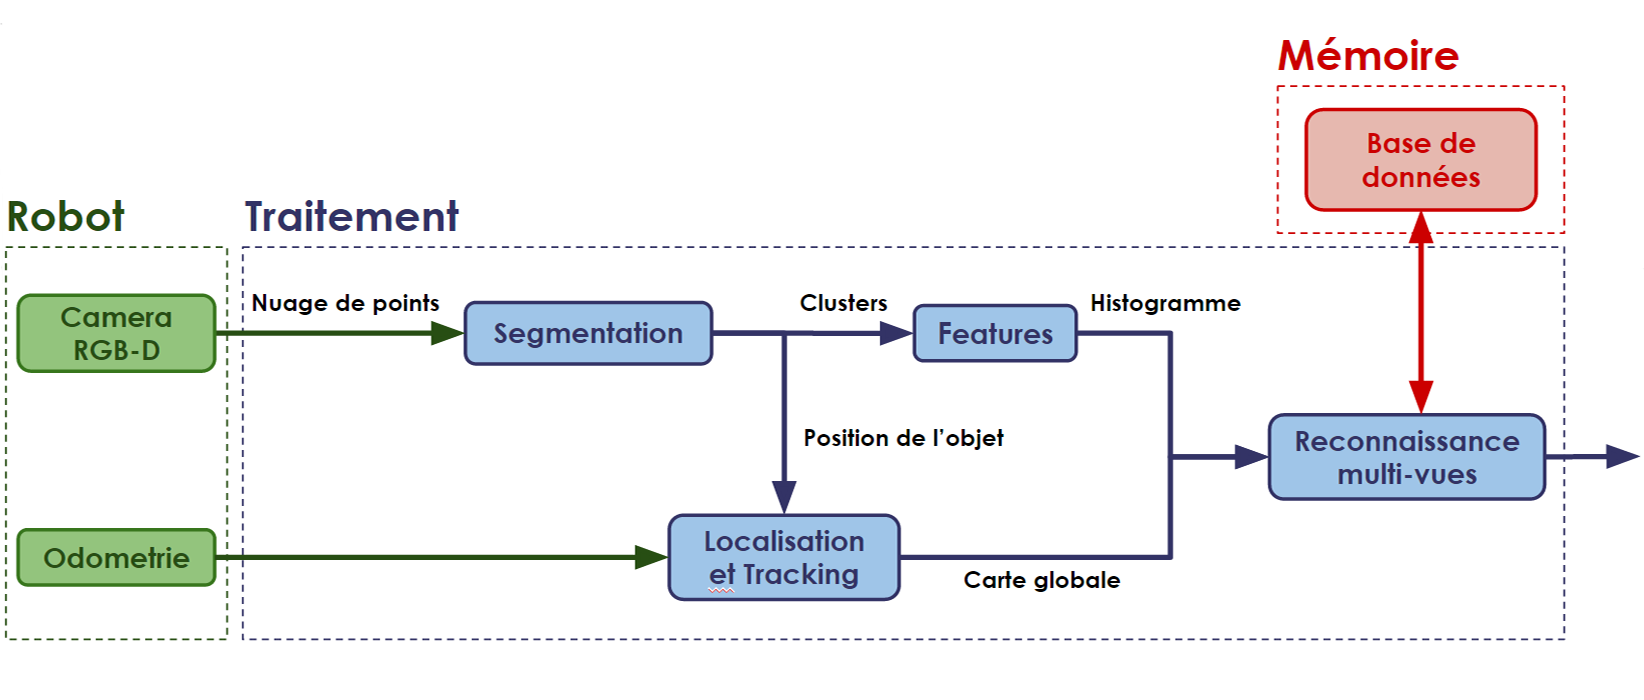
\includegraphics[width=0.95\textwidth]{gen_arc.png}
  \caption{Architecture générale du système}
  \label{fig:architecture}
\end{figure}

Plus précisément, l'unité de traitement reçoit un nuage de points brut provenant de la caméra, ainsi que la mesure de rotation de roues du robot. La première partie du traitement vise à nettoyer le nuage en segmentant des points des objets candidats de la scène, ce qui permet d'enlever une partie non pertinente et de créer un nuage de point dédié pour chaque objet de l'image. Ces nuages de points sont envoyés à l'unité d'extraction de features pour générer des histogrammes représentatif de chaque objets dans l'image. Simultanément, une conversion de référentiel localise des objets dans le repère absolu de déplacement du robot. Puis, les positions des objets sont données au module de localisation et tracking qui suit les observations et les associes entre elles pour avoir une cohérence globale des positions. En dernier lieu, pour chaque objet, les histogrammes de features ainsi que leurs positions converties dans un repère global sont envoyées au module de reconnaissance, et sont utilisés pour reconnaitre les éléments de la scène et donner leur vue la plus probable à chaque instant de temps. 

Les prochaines sections détaillent l'architecture présentée à l'image \ref{fig:architecture}, en présentant le fond théorique derrière le fonctionnement de chaque sous-module.

\section{Segmentation}

La segmentation consiste à isoler des objets dans une image brute, ou en d'autres termes, différencier les éléments qui ne constituent pas un objet et les objets eux-mêmes. La segmentation d'objets est considérée comme un élément essentiel en traitement d'image étant donné qu'une fois l'objet séparé du fond, la reconnaissance devient beaucoup plus simple. La difficulté majeure d'un tel algorithme sur des images RGB vient du fait que la projection de la scène sur le plan image supprime l'information de profondeur. Les capteurs stéréoscopiques et infra-rouges permettent de compenser cette absence d'information et simplifient énormément le traitement nécessaire.

Dans le cas où le capteur est immobile, on utilise classiquement des méthodes de soustraction de fond pour l'étape de segmentation \cite{dai2006prospects}. Ceci n'est pas possible dans notre cas car le robot évolue dans son environnement. La démarche proposée par la littérature dans ce cas considère les objets comme des ensembles de points délimités par un seuil de proximité. Cette définition est suffisamment générale pour permettre de représenter une grande quantité d'objets. Néanmoins, définir ces ensembles dans une image brute n'est pas forcément simple. Par conséquent, on utilise un nouvel \textit{a priori} qui spécifie que les objets se situent sur des plans de support. Bien que plus restrictif que la définition d'avant, cela permet un segmentation crédible. Parmis les méthodes de segmentation se basant sur cette définition, on peut citer Tabletop object detector \cite{tabletop} qui détermine le plan principal de l'image (généralement une table ou le sol) grâce à l'algorithme RANSAC \cite{fischler1981random}, puis recherche des objets dans l'enveloppe convexe de ce plan. Par ailleurs, Caron et al. \cite{caron2014neural} ont proposé une approche légèrement différente. En partant du même principe, le sol est estimé, puis un traitement pour le fond de la scène est appliqué, où les plans orthogonaux à la normale du sol et de taille suffisamment grands sont considérés comme des murs, et les éléments trop près des bords ne sont pas considérés. 

\subsection{Algorithme}

La méthode de segmentation utilisée dans notre cas est celle proposée par Caron et al. Cette méthode s'applique surtout pour de la segmentation d'objets posés sur le sol dans des environnements intérieurs et répond aux exigences du domaine de déplacement du robot : le laboratoire de Thales Theresis.\\

Plus spécifiquement, elle peut être découpée selon les étapes suivantes :
\begin{enumerate}[start=0]
\item Calibration permettant d'obtenir l'équation du sol avant le début de la séquence.
\item Soustraction du sol à partir de l'équation trouvée
\item Filtrage des points trop éloignés, considérés comme plus incertains
\item Calcul de la normale des surfaces de la scène
\item Élimination de murs, considérés comme des grands plans orthogonaux au sol
\item Voxelisation des points non filtrés pour accélérer le traitement
\item Projection des points voxelisés dans le plan du so
\item Regroupement des points en objets grâce à l'algorithme de \textit{clustering} point growing de PCL
\item Calcul du centroïde et des bounding boxes 2D et 3D de chaque objet
\end{enumerate}

Ainsi, l'algorithme fournit la position de chaque objet dans le repère de la caméra ainsi que le nuage de point et les normales qui leur sont associés.

Une calibration initiale est nécessaire pour définir l'équation du sol. Pour cela, on place le robot dans un endroit où l'image obtenue correspond majoritairement au sol. L’équation du plan dominant est extrait par RANSAC et sauvegardée dans un fichier texte. %Une explication plus détaillée sur les sous-méthodes utilisées pour chaque étape est présentée dans les annexes, ainsi qu'une discussion sur les paramètres utilisés.


\subsection{Restrictions} 
La physique des capteurs restreint le type d'objets qui peuvent être aperçus et segmentés, soit à cause des réflexions des rayons infra-rouges, soit à cause de la
résolution limitée des images mesurées. D'un autre côté, la segmentation a ses propres contraintes en ce qui concerne le positionnement des objets dans l'image et, principalement, la définition du sol et des murs. Par conséquent, les restrictions de l'algorithme sont les suivantes :

\begin{itemize}
\item Le sol où le robot se déplace n'est pas accidenté.
\item L'objet se trouve par terre à une distance inférieure à 3 mètres .
\item La lumière ambiante ne doit pas contenir trop de lumière infra-rouge.
\item L'objet n'est ni transparent ni trop réflectif et dépasse le seuil d'appartenance au sol.
\end{itemize} 

Un grand nombre d'objets, entre autres chaises, tables, écrans, boîtes en carton, poubelles, de tailles et formes variés ont été testés et peuvent être segmentés malgré les restrictions. Une exemple de segmentation est présenté dans la figure \ref{fig:mono_recon} pour illustrer la capacité de segmentation. 

\section{Descripteurs}


Le travail des descripteurs est, d'une part, d'extraire des caractéristiques intéressants de l'élément observé et, d'autre part, de réduire la
dimensionnalité de l'espace traité, tout en restant robuste à des transformations affines et aux changements de luminosité. On s'intéresse surtout ici aux descripteurs basés sur le nuage de point des objets, bien qu'il soit possible aussi d'utiliser des descripteurs associés à la texture ou à la couleur. Les descripteurs qui nous intéressent sont des descripteurs géométriques qui essaient de traduire les idées de courbure, de forme et taille dans les histogrammes, et sont intéressants pour étudier les ambiguïtés de reconnaissance. Parmis les descripteurs 3D proposés dans la littérature, on peut citer FPFH \cite{rusu2009fast} qui est invariant par changement de point de vue, SHOT \cite{tombari2010unique} étant un descripteur local de courbure et des descripteurs semi-globales orientés au traitement des occlusions CVFH \cite{aldoma2011cad} et Our-CVFH \cite{aldoma2012our}. Une description détaillée de ces descripteurs et leurs principales différences sont expliquées dans les annexes \ref{annexe:descripteur}. Nous choisissons d'utiliser le descripteur \textit{Viewpoint Feature Histogram} - VFH, car il permet de discriminer non seulement les formes géométriques (pour la reconnaissance d'objet), mais aussi les points de vues (reconnaissance de vue).

En partant de l'hypothèse que la segmentation propose un découpage correct des objets, on extrait des descripteurs globaux à partir des ensembles de points proposés. Ainsi, pour chaque objet, on obtient un histogramme VFH représentatif de l'objet et de la vue segmentée.

\section {Reconnaissance mono-vue} 
\label{sec:rec_mono}

Afin de reconnaitre les objets et leur points de vue rencontrés par le robot, nous utilisons les histogrammes de descripteurs VHF et une base de donnée réalisée à l'avance. Dans cette base, les histogrammes de plusieurs objets sont calculés pour plusieurs points de vues ainsi que leurs positions relatives (Plus de détails sur la construction de la base à la section \ref{sec:base_donnees}). Le but est de retrouver l'objet et son point de vue le plus proche par rapport à la base. Pour cela, il est possible d'utiliser des algorithmes de \textit{machine learning} classiques, mais les résultats sur des réseaux de neurones n'ont pas été très concluants. Aldoma et al. \cite{Aldoma2012} suggèrent l'utilisation de la mesure de similarité entre histogrammes chi-squared, associée au classificateur \textit{k plus proches voisins}, ou K-NN. Le gros avantage de ce classificateur est l'étape d’apprentissage, qui correspond à création d’un arbre de recherche construit à partir de la comparaison croisée entre les éléments de la base. Par rapport aux données dont nous disposons, cet arbre se construit et fournit une estimation du plus proche voisin de manière presque instantannée.

L'API de la librairie FLANN sur PCL permet l'utilisation directe du classificateur K-NN. L'implé- mentation permet l'utilisation de plusieurs définitions de distance entre histogrammes. La définition par défaut, Chi-squared, dont la formule est donnée à l'équation \ref{eq:chi-square}, semble être capable de bien différencier les histogrammes d'entrés, $H_1$ et $H_2$, et a été choisie pour notre système.
\begin{equation}
d(H_1, H_2) = \sum _I \frac{\left(H_1(I)-H_2(I)\right)^2}{H_1(I)}
\label{eq:chi-square}
\end{equation}

\begin{figure}[H]
	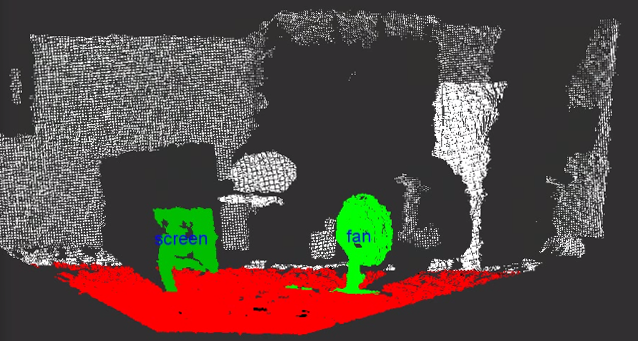
\includegraphics[width=\textwidth]{mono_recon.png}
	\caption{\textbf{reconnaissance mono-vue} - Le résultat de la classification sur les objets segmentés où une écran et un ventilateur étaient reconnus. En rouge le plan du sol et en blanc les points à plus de 3 mètre considérés comme plus bruités. Un remarque pour les ombres infra-rouges qui occultent les objets}
	\label{fig:mono_recon}   
\end{figure}

\section{Localisation et suivi d'objet}

\subsection{Définition de repères}

Se placer dans différents repères permet d'avoir des référentiels plus naturels pour chaque type de composant du robot et pour les objets placés dans la scène. On définit quelques repères et conventions de base pour faciliter la localisation. D'abord le repère de la base du robot est orthonormale positif, où le déplacement vers l'avant correspond à l'axe $\vec{x}$, vers la gauche à l'axe $\vec{y}$ et vers le haut à l'axe $\vec{z}$. Un deuxième référentiel utilisant les mêmes conventions positionne le capteur RGB-D par rapport au robot. Enfin, le dernier référentiel correspond au repère optique du capteur orienté selon la convention usuelle pour les images avec l'axe $\vec{x}$ orienté vers la droite, l'axe $\vec{y}$ vers le bas et enfin l'axe $\vec{z}$ vers l'avant. Ces trois repères permettent d'orienter tous les éléments aperçus par le robot dans l'environnement de façon pratique.

Une méthode de transformation entre repères permet ensuite le passage de l'un à l'autre. On peut ainsi obtenir la position de l'objet  dans le repère global d'après sa détection par la caméra. La transformation entre une base $a$ et une autre $b$ est faite par une matrice de transformation classique, décrit par l'équation \ref{eq:mat_rotation}. 

\begin{equation}
	\mathbf{R}^{a}_{b} = 
	\begin{bmatrix} 
	 	\cos \theta &  -\sin \theta & \Delta x \\ \sin \theta & \cos \theta & \Delta y \\ 0 & 0 & 1
	 \end{bmatrix}
	\label{eq:mat_rotation}
\end{equation}

où $\theta$ équivaut à l'angle entre les deux repères et $\Delta x$ et $\Delta y$ sont les translations linéaires entre eux.

\subsection{Bases mobiles}

\subsubsection{Estimation de l'odométrie}

Certains robots sont dotés de capteurs capables d'estimer de façon
approximative son dépla-cement. C'est aussi le cas du robot utilisé qui
possède des roues codeuses capables d'estimer la rotation angulaire des
roues. Pour le cas d'un robot différentiel, où chaque roue peut être
commandée indépendamment, le déplacement et l'orientation suit les équations suivantes:

\begin{equation}
	\begin{array}{rcl}
		\delta x_t &=& \delta s_t \cdot cos(\theta_{t-1}) \\
		\delta y_t &=& \delta s_t \cdot sin(\theta_{t-1}) \\
		\delta \theta_t &=& \frac{\delta \omega_{g} + \delta \omega_{d}}{d_{r}}\\
		\delta s_t &=& \frac{\delta \omega_{g} + \delta \omega_{d}}{2}						
	\end{array}
\end{equation}
$\omega_g$ et $\omega_d$ sont des respectives variations angulaire des roues et $d_r$ est la distance entre elles. Une intégration, au sens mathématique \ref{eq:integ}, de la différence entre
l'odométrie entre deux intervalles de temps permet de retrouver la position global du robot.

\begin{equation}
	\begin{array}{rcl}
		x_t &=& x_{t-1} + \delta x_{t} \times cos(\theta_{t-1}) - \delta y_{t} \times sin(\theta_{t-1}) \\
		y_t &=& y_{t-1} + \delta x_{t} \times sin(\theta_{t-1}) + \delta y_{t} \times cos(\theta_{t-1}) \\
		\theta_t &=& \theta_{t-1} + \delta\theta_{t}
	\end{array}
	\label{eq:integ}
\end{equation}

\subsection{Filtre de Kalman }

Afin de pouvoir utiliser le déplacement du robot par rapport aux objets pour les identifier, il est d'abord nécessaire de les localiser et les suivre. À cause
de la divergence de l'odométrie, l'imprécision de la segmentation et le calcul
du centroïde de l'objet, la position estimée est fortement bruitée et rend la suivie et identification infaisable
lorsque plusieurs objets sont trop proches. Nous utilisons donc un filtre de Kalman pour corriger cette erreur de mesure et fournir une estimation plus fiable de la position des objets.

Classiquement le filtre de Kalman est mis à jour selon deux étapes : 

\subsubsection{Prédiction} Une première de prédiction qui utilise le modèle linéaire $\textbf{F}_{k}$ pour décrire l'évolution des états au long du temps avec son bruit de process, $\textbf{Q}_{k}$, associé et qui estime \textit{a priori} la covariance de l'erreur $\textbf{P}_{k|k-1}$. Formellement, on utilise les équations \ref{eq:kalman_prediction}

\begin{equation}
	\begin{array}{ccl}
		\hat{\textbf{x}}_{k|k-1} &=& \textbf{F}_{k}\hat{\textbf{x}}_{k-1|k-1} + \textbf{B}_{k} \textbf{u}_{k-1}\\
		\textbf{P}_{k|k-1} &=& \textbf{F}_{k} \textbf{P}_{k-1|k-1} \textbf{F}_{k}^{T} + \textbf{Q}_{k}
	\end{array}
	\label{eq:kalman_prediction}
\end{equation}

\noindent Où les variables sont :\\
$\textbf{F}_{k}$ : la matrice de dynamique du système définie comme identité dans notre cas, si l'on considère que l'objet reste immobile\\
 $\textbf{u}_{k}$ : l'entrée de commande, nulle dans notre cas\\
 $\textbf{B}_{k}$ : la matrice qui relie l'entrée de commande $u$ à l'état $x$, nulle également\\
$\textbf{P}_{k|k-1}$ : la matrice d'estimation a priori de la covariance de l'erreur \\
$\textbf{Q}_{k}$ : la matrice de covariance du bruit de process, diagonale dans notre cas.\\

\noindent Avec: \\
$\textbf{z}_{k}$ \space \space: observation ou mesure du process à l'instant k \\
$\textbf{H}_{k}$ \space : matrice qui relie l'état $\textbf{x}_{k}$ à la mesure$ \textbf{z}_{k}$\\
$\textbf{P}_{k|k}$ : matrice d'estimation a posteriori de la covariance de l'erreur\\
$\textbf{R}_{k}$ \space \space : matrice de covariance du bruit de mesure

\subsubsection{Innovation}
Une deuxième mise à jour, où l'observation est incorporée dans le calcul de l'innovation, $\tilde{\textbf{y}}_{k}$, et du gain de Kalman, $\textbf{K}_{k}$ est décrite par l'équation \ref{eq:innovation}.

\begin{equation}
	\begin{array}{ccl}
		\tilde{\textbf{y}}_{k} &=& \textbf{z}_{k} - \textbf{H}_{k}\hat{\textbf{x}}_{k|k-1} \\
		\textbf{S}_{k} &=& \textbf{H}_{k}\textbf{P}_{k|k-1} \textbf{H}_{k}^{T}+\textbf{R}_{k} \\
		\textbf{K}_{k} &=& \textbf{P}_{k|k-1}\textbf{H}_{k}^{T}\textbf{S}_{k}^{-1} \\
		\hat{\textbf{x}}_{k|k} &=& \hat{\textbf{x}}_{k|k-1} + \textbf{K}_{k}\tilde{\textbf{y}}_{k} \\
		\textbf{P}_{k|k} &=& (I - \textbf{K}_{k} \textbf{H}_{k}) \textbf{P}_{k|k-1}
	\end{array}
	\label{eq:innovation}
\end{equation}
\noindent Avec :\\
 $\textbf{z}_{k}$ : l'observation s'agit de la position de l'objet segmenté dans le repère absolu\\
$\textbf{H}_{k}$ : la matrice qui relie l'état $\textbf{x}_{k}$ à la mesure $ \textbf{z}_{k}$ : Ici, il s'agit d'une matrice identité puisque tout est réalisé dans le repère absolu.\\
$\textbf{P}_{k|k}$ : la matrice d'estimation \textit{a posteriori} de la covariance de l'erreur\\
$\textbf{R}_{k}$ : la matrice de covariance du bruit de mesure. Matrice diagonale dans notre cas.

\subsubsection{Suivi multi-cibles}
Le caractère monomodal du filtre de Kalman nous contraint à ne pouvoir suivre qu'un seul objet à la fois. Pour obtenir un suivi multimodal, il faut que plusieurs filtres tournent en parallèle. Ainsi, le problème passe d’estimer la position d'un seul objet à celui de décider quelle observation appartient à quel filtre. Pour ce faire, nous définissions une matrice de distances entre chaque nouvelle observation et les états courants de chaque filtre de Kalman déjà créé.
Ensuite, les nouvelles observations sont utilisées pour mettre à jour les filtres de Kalman dont l'estimation est la plus proche selon cette matrice. Avant toute mise à jour, on vérifie que la distance entre l'observation et l'estimation du filtre ne dépasse pas un certain seuil. Pour chaque observation qui n'a pas pu être associée à un filtre déjà existant, on crée alors un nouveau filtre.

\section {Reconnaissance Multi-vue}

\subsection {Chaînes de Markov Cachées}

Le déplacement physique du robot produit une séquence
d'observations, sous différents points de vues, d'un même objet. On exploite
l'information odométrique entre les différentes vues pour renforcer l'estimation de la vue d'un objet. De cette manière, l'évolution de la
reconnaissance au cours du temps est représentée par un processus
stochastique, dont une modélisation possible consiste à le traiter
de façon discrète dans un espace d'état. Ayant l'apriori que la
dernière image et le dernier déplacement suffisent pour faire cette
prédiction (c'est-à-dire en respectant la propriété de Markov de premier
ordre), le processus stochastique est modélisée par une
chaîne de Markov cachée.

Concrètement, les états cachés correspondent à des vues d'objets connus au
préalable et déjà stockés dans la mémoire du robot. Cela contraint le
nombre d'états et garantie que la chaîne soit finie. Puis, une
matrice de transition, $a_{i,j}$, décrit l'évolution du processus. C'est cette matrice de transition qui permet de prendre en compte l'odométrie et la transition entre les vues d'un même objets. Enfin, une autre matrice, $\mathrm{P}\big( y_1 \ | \ k \big)$, dite matrice d'émission, estime la vraisemblance entre l'observation
et les états de la chaîne.

Plus précisément,  $a_{i,j}$ est définie en fonction de l'angle $\delta_{angle}$, calculé par \ref{eq:delta_ang} qu'a parcouru le robot par rapport à l'objet entre deux vues successives. Dans notre modèle, on considère que $a_{i,j}$ est nulle si $i$ et $j$ sont deux vues d'objets différents. Pour deux vues $i$ et $j$ d'un même objet, séparées d'une distance $d$, le poids accordé à $a_{i,j}$ sera d'autant plus fort que $\delta_{angle}$ et $d$ sont proches. D'autre part, la matrice d'émission $\mathrm{P}\big( y_1 \ | \ k \big)$ correspond à la similarité entre l'histogramme d'un objet segmenté $y$ et celui d'une vue d'objet dans la base de données $k$, normalisés par l'équation \ref{eq:dist_norm}. La similarité est calculée comme l'inverse de la distance Chi square définie à la section \ref{sec:rec_mono}.
  \begin{equation}
  \begin{array}{rcl}
    \vec{d}_0 &=& p_0 - p_{obj}\\
    \vec{d}_1 &=& p_1 - p_{obj} \\
     \delta_{angle} &=& atan(\vec{d}_1) - atan(\vec{d}_0)
  \end{array}
  \label{eq:delta_ang}
  \end{equation}
La transformation des distances des histogrammes en probabilité est faite d'après la normalisation suivant :
\begin{equation}
	\mathbb{P}(y|x, database) = \frac{\sum_a d_a^x - d_y^x}{\sum_b \sum_c d_c^x - d_b^x}
	\label{eq:dist_norm}
\end{equation}
où $x$ est l'image de teste et y un élément de la base de donné. Dans le cas du plus proches voisin la normalisation prend en compte seulement les k plus proches histogrammes, en contraste au approche \textit{bruta force}.

Une autre modélisation possible aurait été d'avoir une chaîne de Markov
cachée distincte pour chaque objet et ensuite décider à chaque pas de temps le
processus le plus vraisemblable. Cette modélisation peut être vue comme un sous-ensemble du cas
précédent où les transitions entre deux objets ne sont pas
considérées. Pourtant, il peut arriver que deux objets soit considérés comme positionnés au même endroits, ou bien que des objets mobiles fusionnent (par exemple, une personne qui viendrait s'asseoir sur une chaise, ou encore un personne
qui commence à marcher) \footnote{Le fait de se mettre en mouvement
  altère les formes d'une personne, ce qui rend possible sa détection
  comme un nouvel objet.}.

\subsection{Algorithme de Viterbi}

Reste donc à extraire des informations de la modélisation Markovienne proposée.
La séquence d'états la plus vraisemblable qui pourrait avoir géneré
les observations  $y_1,\dots, y_T$, correspond normalement à la séquence d'objets reconnus.
Afin de retrouver cette séquence, aussi appellée chemin, on fait 
appel à la programmation dynamique, et plus spécifiquement à l'algorithme de Viterbi, d'où le nom chemin de Viterbi.
L'algorithme retrouve de façon récursive l'état courant le plus probable, en
prenant en compte seulement les observations jusqu'à un instant donné et son
estimation aux instants antérieurs. Ceci se traduit par les équations \ref{eq:viterbi}

\begin{equation}
  \begin{array}{rcl}
    V_{1,k} &=& \mathrm{P}\big( y_1 \ | \ k \big) \cdot \pi_k \\
    V_{t,k} &=& \max_{x \in S} \left(  \mathrm{P}\big( y_t \ | \ k \big) \cdot a_{x,k} \cdot V_{t-1,x}\right)
  \end{array}
	\label{eq:viterbi}
\end{equation}

Ici, $V_{t,k}$ représente la probabilité que la séquence d'états la plus probable finisse dans l'état $k$, ayant généré les observation à l'instant $t$, tandis que $\pi_i$ représente la probabilité initiale de se retrouver en chaque état. Pour retrouver le chemin de Viterbi, il suffit de trouver le maximum de $V_{t,k}$ :

\begin{equation}
  \begin{array}{rcl}
    x_T &=& \arg\max_{x \in S} (V_{T,x})
  \end{array}
\end{equation}

\subsection {Graphe d'aspect polaire}
%\celine{Je trouve que cette section n'est pas très utile en fait. Tu fais référence ailleurs à un graphe d'aspect (je ne sais plus où). Si tu veux, tu peux mettre cette partie dans les annexes et y faire référence à l'endroit du rapport ou tu en parles}

On considère que les objets sont décrits par deux dimensions
d'information : une spatiale, représentant la position absolue de l'objet
dans l'environnement ainsi que les positions relatives où l'objet a été
visualisé, et une autre dimension visuelle, donnée par les descripteurs
géométriques, de couleurs et de texture. On cherche à représenter cette description dans un référentiel unique. Le graphe d'aspect permet de coupler
l'ensemble des images suivant ses possibles transitions spatiales, ce qui
résulte dans la possibilité de construire le modèle à la volée et de
jouer avec sa densité d'information - le nombre d'images intégrées au modèle.

\begin{figure}[H]
  \centering
  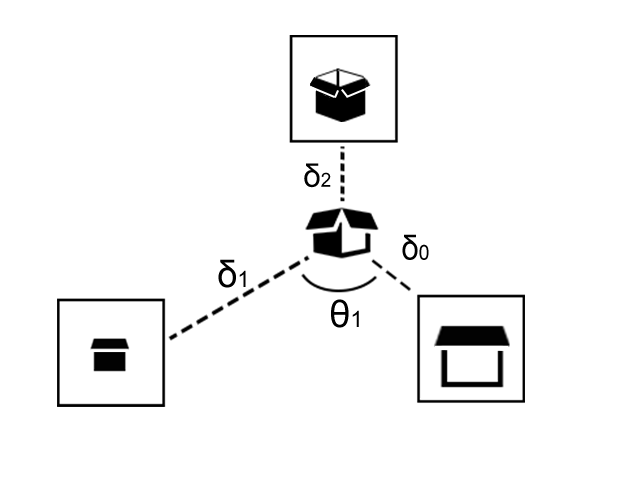
\includegraphics[width=0.4\textwidth]{object_model.png}
  \caption{Représentation des objets par un modèle polaire}
	\label{fig:graphe_polaire}
\end{figure}

Un référentiel polaire entrelace toutes ces informations
de façon à représenter la position spatiale d'où l'observation a été
faite, comme représenté dans l'image \ref{fig:graphe_polaire}. Pour la
construction du modèle les conventions suivantes ont été adoptées :
\begin{itemize}
\item l'angle zéro est attribué à la première observation
\item L'origine du référentiel est la position globale de l’objet
\item Les features sont labellisées d'après le déplacement angulaire
  et la distance au centroïde de l'objet.
\end{itemize}

Une grande majorité des features visuelles ne sont pas invariantes à l'échelle, et ce d'autant plus si la résolution de l’image joue un rôle critique pour la
détection de features, comme les patches SIFTs. Ainsi, prendre également en compte la distance à laquelle l’image a été prise peut être intéressant pour limiter la
classification à une échelle valable.
%%%% Evaluation
\chapter {Protocole Expérimental}

\section{Matériel utilisé}
En ce que concerne les aspects matériels, le robot bimoteur Wifibot v2, équipé d'un ordinateur à bord, sera utilisé comme plateforme mobile. L'acquisition des données est faite par une camera RGB-D Asus Xtion Pro Live. Par rapport au choix logiciel, l'environnement robotique ROS\footnote{Robot Operating System} a été adopté pour avoir les bibliothèques qui permettent de gérer les nuages de points, Freenect, OpenNi2 et PCL\footnote{Point Cloud Library}, et d'autres nombreux outils de contrôle du robot et sauvegarde d'informations.

\section{Setup expérimental}
Pour évaluer les capacités de reconnaissance du robot, vingt objets de tailles et formes diverses ont été choisis pour être incorporé à la base de connaissance. Ils s'agit d'objets typiques qui peuvent être facilement retrouvés dans un laboratoire ou un bureau. Ensuite, nous avons effectué un tour complet de l'objet avec le robot en sauvegardant les nuage de point et en extrayant les features VFH pour huit positions différentes écartées de 45 degrés à 1.5 mètres de distance. La position correspondent à l'angle zéro a été choisie de manière aléatoire en alignant un des axes de l'objet avec celui du capteur. L'image \ref{fig:setup_expe} des vues d'un objet exemplifie la composition de la base de données. Une liste complète des objets figure en annexe \ref{fig:dataset}.

\begin{figure}[H]
	\subfloat{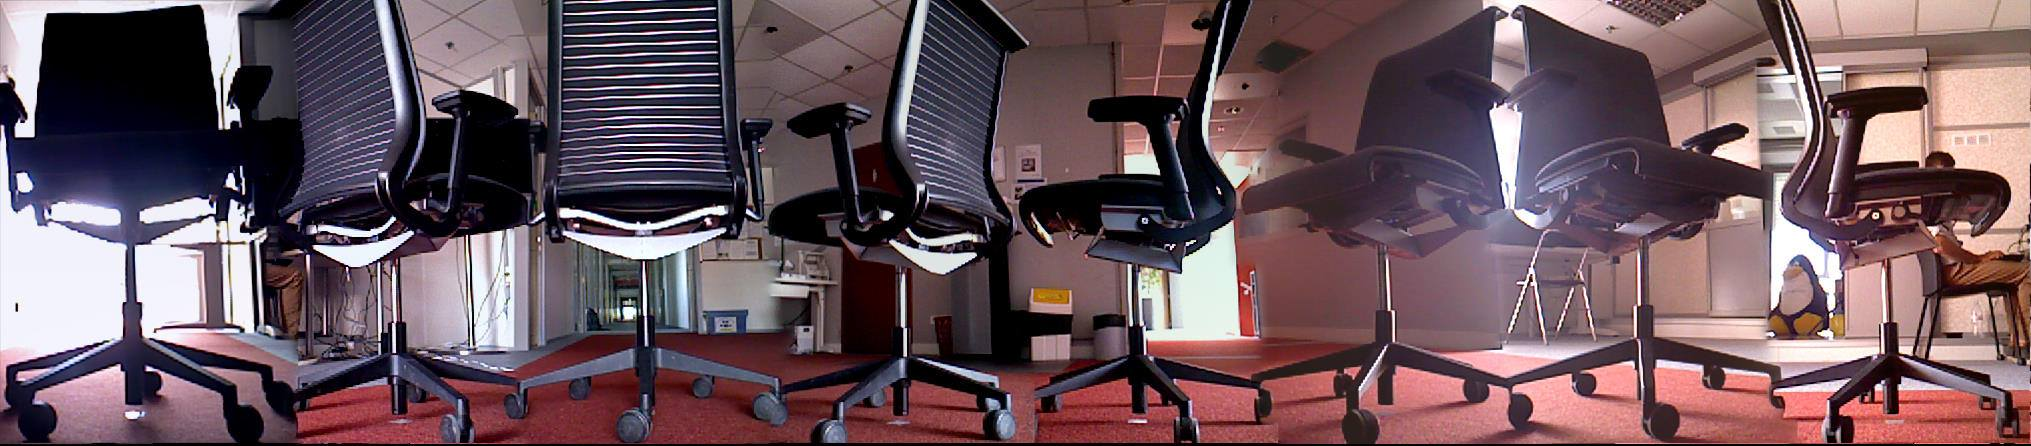
\includegraphics[width=\textwidth]{chair_db.jpg}}		
	\caption{Les huit point de vues de l'objet commençant par la position zéro et en tournant le robot en sens horaire}
	\label{fig:setup_expe}
\end{figure}

\section{Résultats expérimentaux}
\subsection{Comparaison à la reconnaissance mono-vue}
Une première évaluation consiste à faire un tour complet autour de l'objet à reconnaitre pour quatre positions angulaires différentes : $0, 45, 90$ et une dernière choisie de manière aléatoire pour chaque objet. Le robot fait le tour à une vitesse de $0.35 \pm 0.1 m/s$ à une distance de $1.5m$, en enregistrant des images à $1hz$, ansi, une expérience typique est constituée d'environ $25$  images d'angle différent et prendre $25 \pm 3$ seconds. 

La difficulté de l'évaluation vient, premièrement, du fait du robot avoir une base assez discrète ce qui donne marge à des mauvaise reconnaissance mono-vue une fois le point de vue étant inexistant dans la base de connaissance. Puis, la vitesse du déplacement résulte dans images plus floues lors des acquisitions et la modification de l'angle de la caméra\footnote{L'angle entre la base et la tête de la caméra Asus Xtion est facilement modifié.} apportent un obstacle en plus pour le \textit{matching} de descripteurs dans le classificateur K-plus proches voisins.

Un expérience typique est illustrée dans l'image \ref{fig:resultats_expe} :

\begin{figure}[H]
	\subfloat{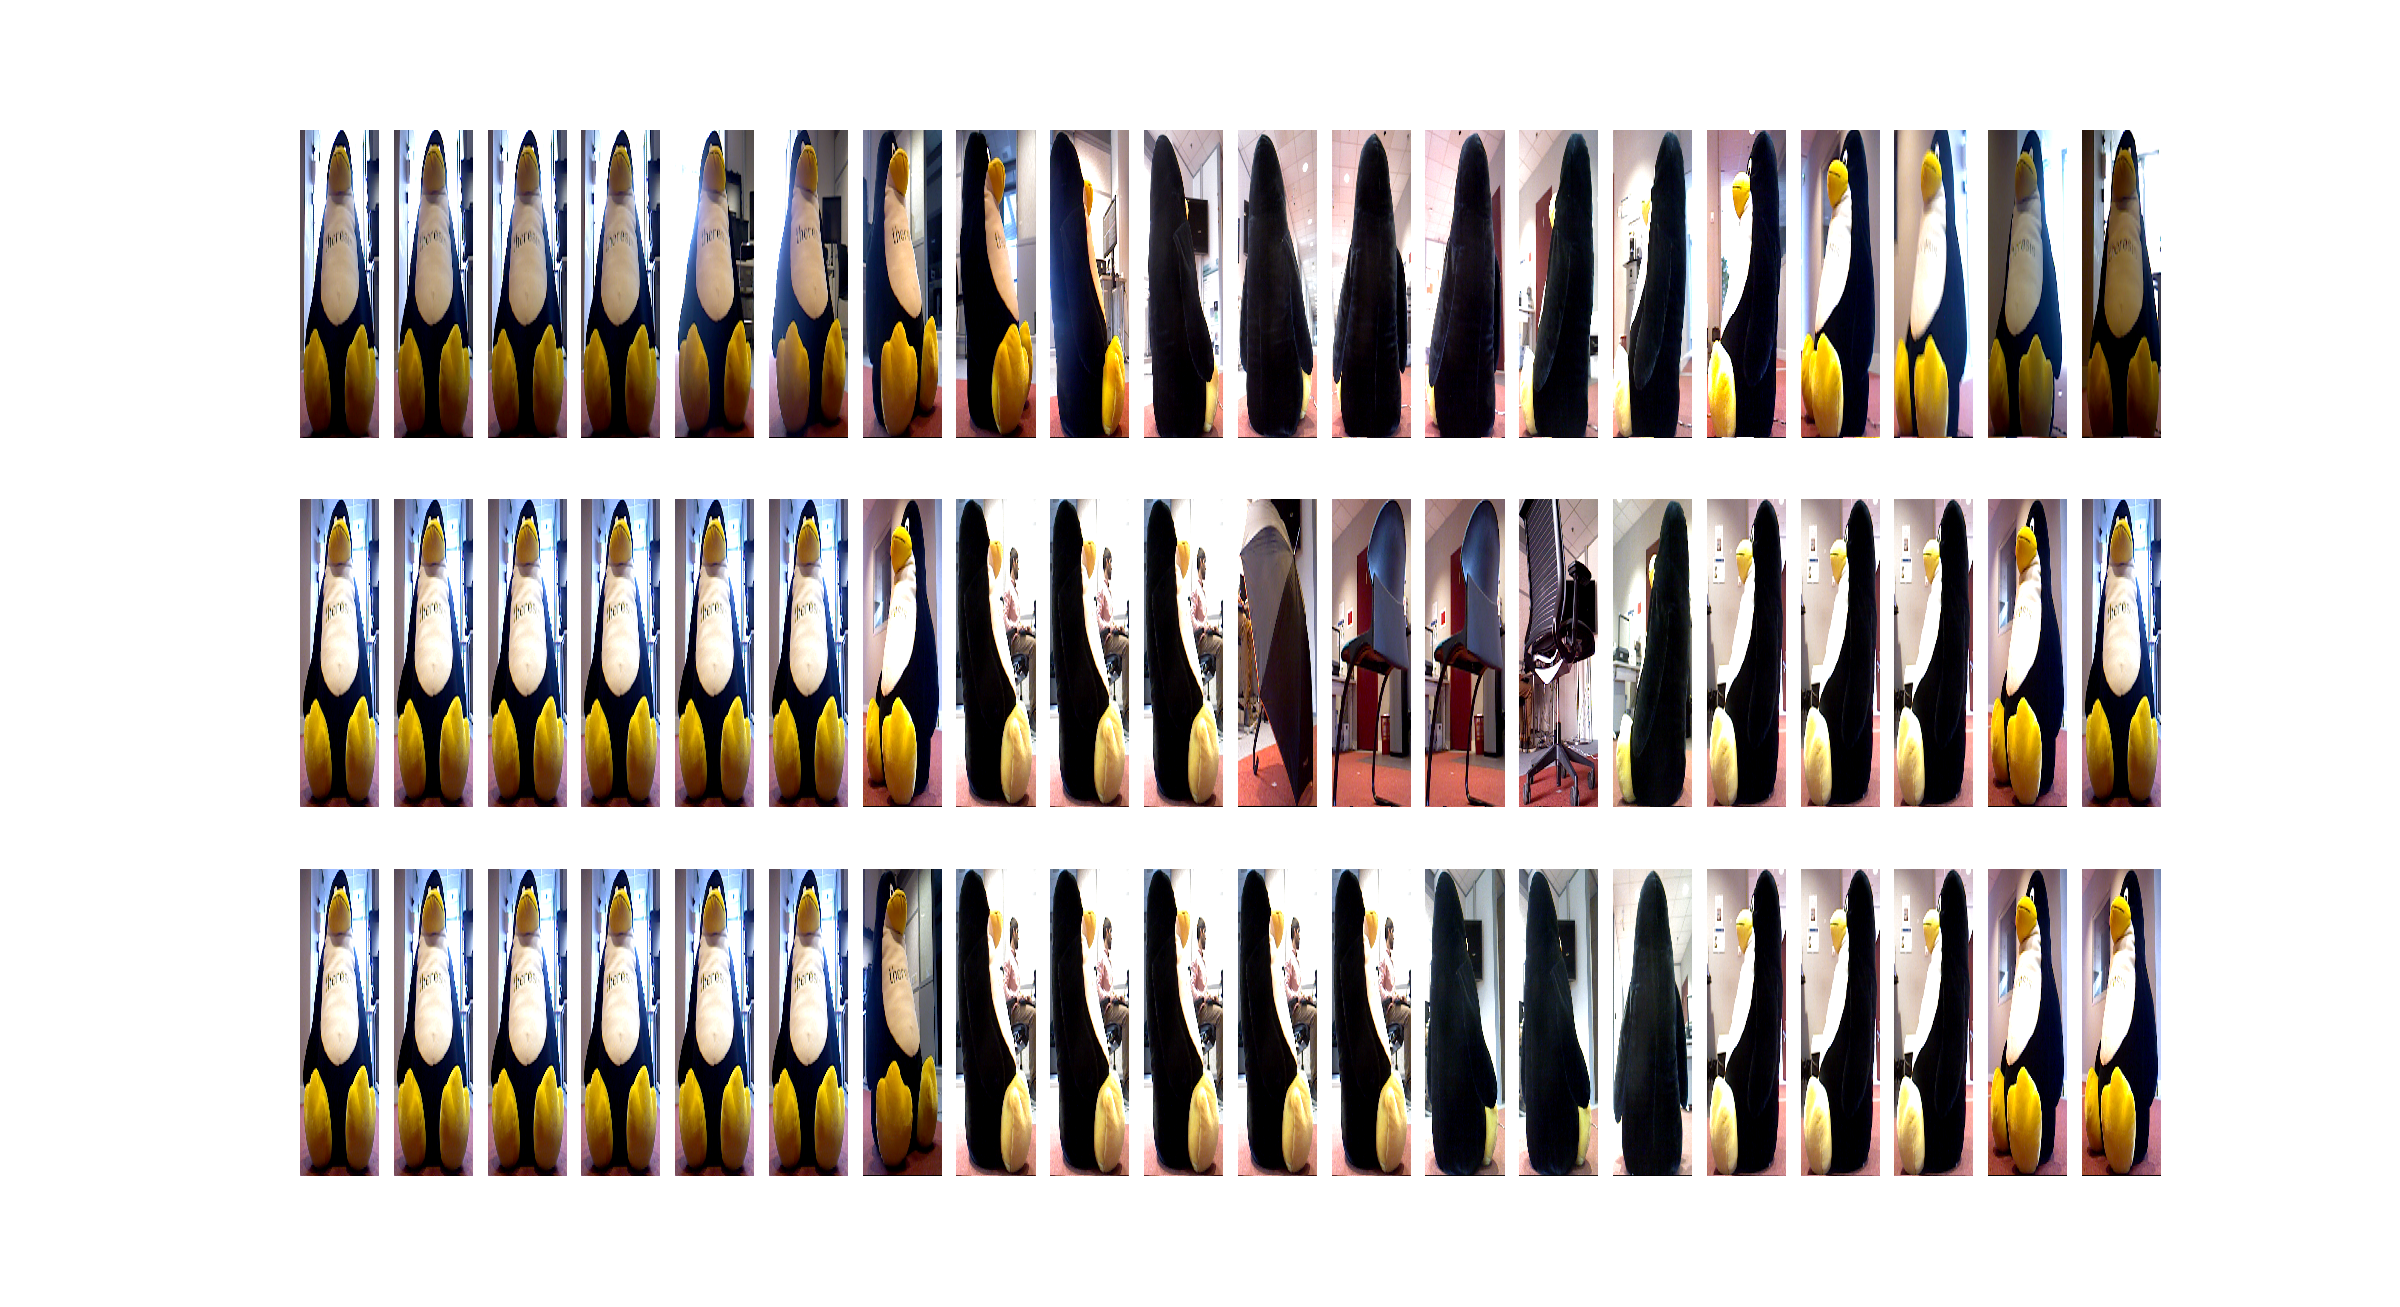
\includegraphics[width=\textwidth]{hmm_example.png}}	
			\caption{\textbf{Résultat de l'évaluation} - Reconnaissance multi-vue corrige des ambiguïtés et surmonte la mauvaise segmentation lors de la création de la base.}
	\label{fig:resultats_expe}
\end{figure}

La première ligne correspond à la séquence d'images vues par le robot à chaque instant de temps, et donc, l'objet à être reconnu. La seconde ligne, donnée par l'algorithme de reconnaissance, équivaut à la vue la plus probable de l'objet reconnue par le K-plus proches voisins. Il est intéressant remarquer que l'invariance à rotation du descripteur trompe l'estimation de l'orientation en prenant son correspond énantiomorphe dans le premier carré rouge. Autrement, le dos du pinguin étant une grande surface presque plane, il est partiellement retiré par l'étape de segmentation. Ainsi, le nuage de points résultant de ce point de vue n'est pas suffisamment complet pour caractériser correctement l'objet, ce qui induit une mauvaise reconnaissance dans le carré bleu. Au final, on remarque que le traitement apporté par la chaîne de Markov cachée permet de corriger les problèmes d'une base de donnée relativement sparse avec des possibles erreus de segmentation, permettant la correction simultanée de la reconnaissance de l'objet et de son orientation en ligne. 

%\begin{figure}[H]
%	\subfloat{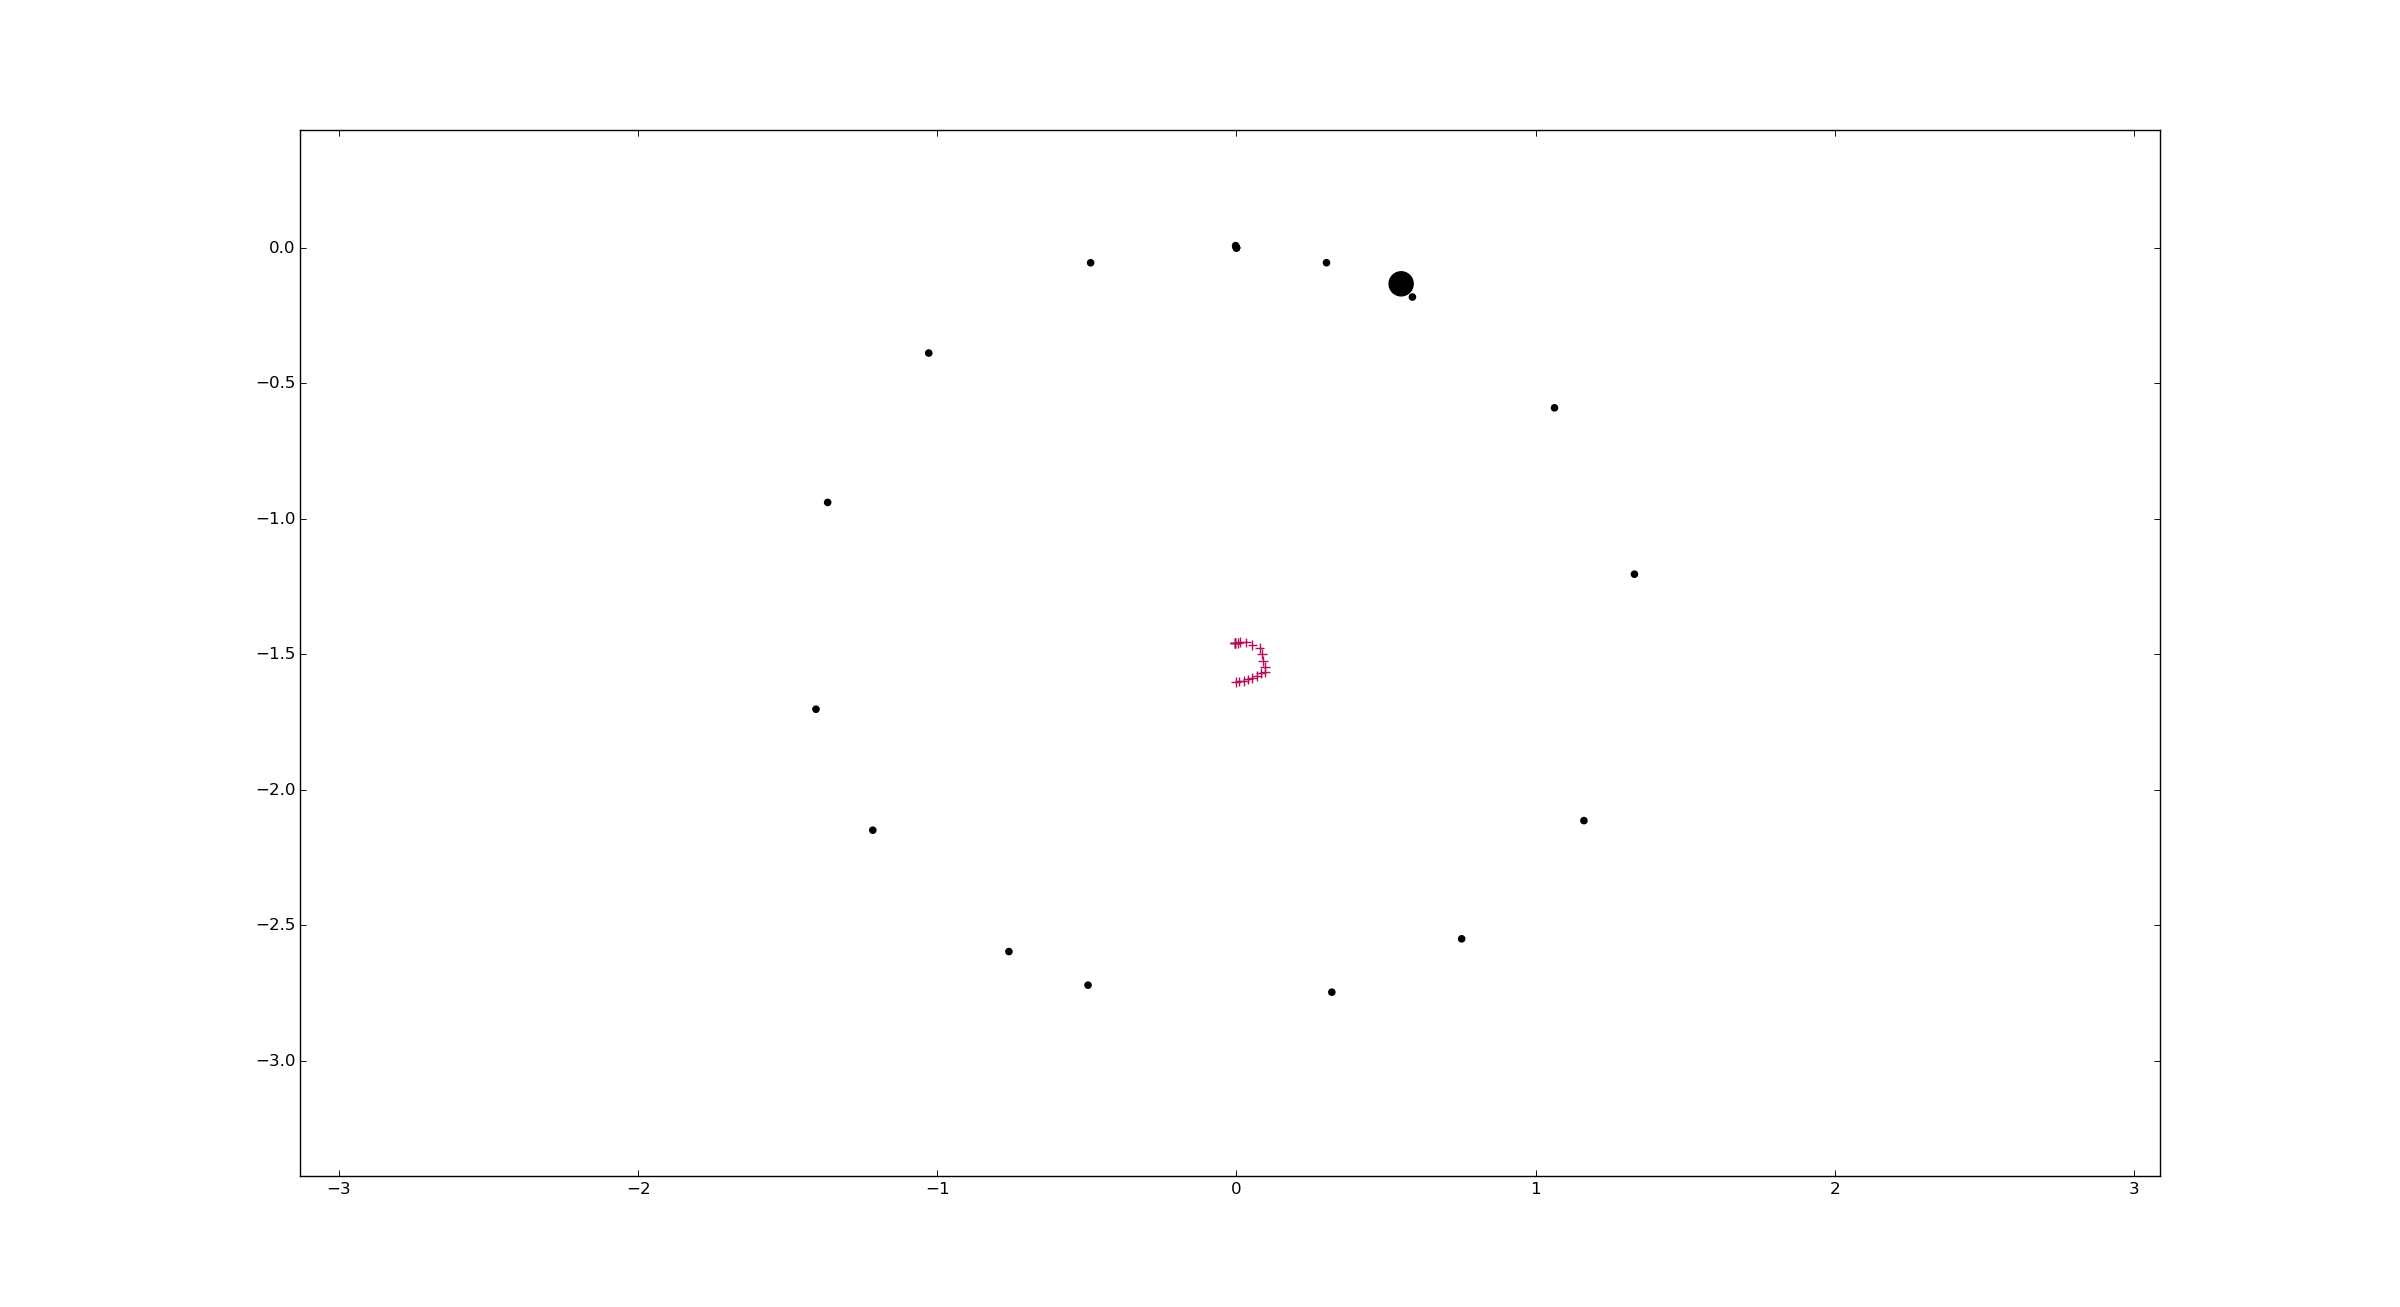
\includegraphics[width=\textwidth]{hmm_mov.png}}		
%\end{figure}


{\color{green}
Dans le premier tableaux on retrouve le résultats de la reconnaissance donné par la comparaison des histogrammes provenant du *plus proche voisin*. Ce résultat estime la capacité de distinguer deux objets quelconques, en autre mots, cette capacité viens de la représentativité des descripteurs utilisés et l'efficacité de la mesure de similarité entre histogrammes.
}

%\subsection{Robustesse à l'occlusion}

\subsection{Suivi et reconnaissance multi-cibles}

Le deuxième expérimentent correspond à placer des objets appris auparavant dans une pièce et conduire le robot faisant en sort qu'il les regardait de plusieurs points de vues différents. 
Ce scénario est beaucoup plus complexe que celui d'avant. D'abord les objets occultent uns aux autres résultant en mauvaises segmentations. Ensuite, la suivi d'objets est plus complexe
La carte finale donnée par l'algorithme, \ref{fig:multi_map}, 

\begin{figure}[H]
	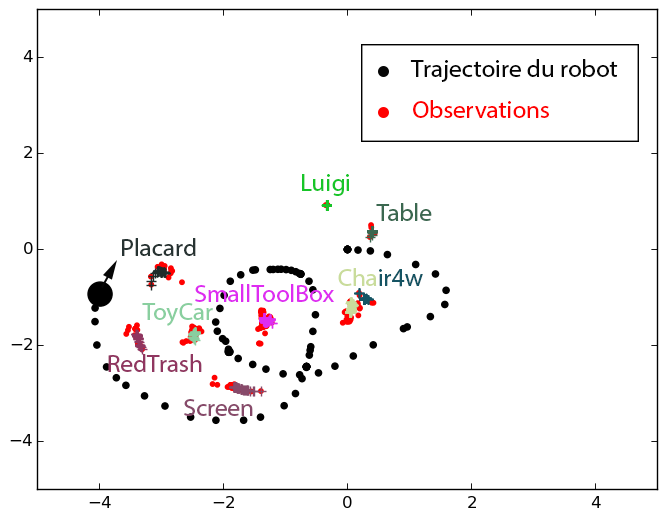
\includegraphics[width=\textwidth]{map.png}
	\caption{...}	
	\label{fig:multi_map}
\end{figure}

\section{Problèmes rencontrés}

\subsubsection{Synchronisation}

\subsubsection{Problèmes de déplacement}

La roulette de support originalement installée avait deux axes de
rotation. Pourtant, quelques mouvements de rotation du robot alignent
la roulette orthogonalement au sens du prochain mouvement ce qui crées
une torche parasite que perturbe la trajectoire voulue. Une tentative
frustrée d'installer une bille omnidirectionnelle à roulement, qui se
bloquait sur la moquette avec le poids du robot, a fait que
l'originale était réinstallée. Une deuxième solution serait d'interdire
certains mouvements du robot pour éviter cette déviation.
%%%% Conclusion
\chapter{Conclusion}

\section{Synthèse} 
La principale contribution de ce projet est liée au traitement de la reconnaissance qui intègre un modèle temporel de transition entre vues. La méthode proposée ici pourrait être mise en place pour n'importe quel système de reconnaissance d'objets à condition qu'il soit mobile et capable de fournir une estimation de son déplacement, et que chaque élément de la base des objets à reconnaitre soit associé à une estimation de son orientation. La reconnaissance d'objets multi-vues augmente la capacité à résoudre des situations ambiguës et gère les problèmes de bruit provenant de la base de donnée (absence de vue, erreurs de segmentation). Elle se montre plus performant quand comparé à son correspondent fixe d'après une première évaluation, ayant un taux de réussit de 92\% lorsqu'un tour complète est fait pour la reconnaissance d'objet, en contraste aux 59\% du système classique. Pour le défi de reconnaître l'orientation spatial le taux diminue mais restant encore assez élévé autour de 75\%.

\section{Discussion} 
Même ayant des résultats intéressants quelques limitations apparaissent lorsqu'on se déplace dans environnement plus exigeants et qu'on veut se déplacer librement. Regarder les objets de trop près, par exemple, coupe une partie de l'objet dans l'étape de segmentation que finit pour être mal classifié dans la suite, ce qui restreint le zones de déplacement ou exige un traitement a priori en plus pour ce cas. De même, objets placés à une distance inférieur à 1 mètre entre eux risquent d'être mélanges par le tracking. Le modèle est, aussi, sensible à la densité de la base de données, car avoir une base trop discrète résulte en points de vues inexistants qui sont souvent mal associés à d'autres objets. 

\section{Perspectives} 
 La formulation de la chaîne de Markov cachée est suffisamment général pour incorporer des nuances plus complexes en cas d'occlusion, de changement ou d'association d'objet (humain+chaise). Explorer ce potentiel semble agrandir encore plus la puissance du modèle. Au même temps,la communication entre la reconnaissance, qui suggérait des modèle cinématiques de déplacement, et le module de suivi multi-cible peut faire en sort que environnements plus complexes avec des objets mobiles où la position physiques des objets, des fois, n'est pas suffisant pour les déterminer puissent être gérés. Une amélioration un peu plus immédiate serait d'ajouter des features de couleur et de texture pour lever les ambiguïtés de vues.  Finalement intégrer un algorithme de SLAM pour rendre plus robustes les estimations de position et avoir une meilleure représentation de l'environnement couplé avec un méthode de planification de trajectoires afin que le robot puisse se déplacer de manière autonome. Par ailleurs, on peut envisager une extension du filtre de Kalman pour des objets en déplacement grâce à des modèles cinématiques suggérés par la reconnaissance.








% \listoffigures
% \listoftables
%%%% Bibliografia 
% \bibliographystyle{ieeetr.bst}
% \bibliography{rapport}

%%%% bibliografie
\chapter{Bibliographie}

[1]Hermann Borotschnig, Lucas Paletta,Manfred Prantl and Axel Pinz 
Active Object Recognition in Parametric Eigenspace 
Submitted to BMVC98, Southampton, United Kingdom, 14-17 Sept. 1998 \\

[2] View-based dynamic object recognition based on human perception \\

[3] L.-C. Caron, D. Filliat, A. Gepperth.
Neural Network Fusion of Color, Depth and Location for Object Instance Recognition on a Mobile Robot. 
Second Workshop on Assistive Computer Vision and Robotics (ACVR), in conjunction with European Conference on Computer Vision, Sep 2014, Zurich, Switzerland.\\

[4] Radu Bogdan Rusu, Gary Bradski, Romain Thibaux, John Hsu,
Fast 3D Recognition and Pose Using the Viewpoint Feature Histogram \\

[5] G. Burel and H. Henocq
Three-dimensional invariants and their application to object recognition
Signal Process., vol. 45, no. 1, pp.1–22, 1995. \\

[6] A. Johnson and M. Hebert
Using spin images for efficient object recognition in cluttered 3D scenes
IEEE Transactions on Pattern Analysis and Machine Intelligence, May 1999. \\

[7] T. Gatzke, C. Grimm, M. Garland, and S. Zelinka 
Curvature Maps for Local Shape Comparison,” 
in SMI ’05: Proceedings of the International Conference on Shape Modeling and Applications 2005 (SMI’05), 2005, pp. 246–255. \\

[8] R. B. Rusu, N. Blodow, and M. Beetz, “Fast Point Feature Histograms
(FPFH) for 3D Registration,” in ICRA, 2009. \\

[9] B.-C. M. and G. C., “Characterizing shape using conformal factors,”
in Eurographics Workshop on 3D Object Retrieval, 2008. \\

[10] K. Lai, L., X. Ren, \& D. Fox  A Large-Scale Hierarchical Multi-View RGB-D Object Dataset In IEEE International Conference on Robotics and Automation (ICRA), May 2011. \\

[11] R. B. Rusu and S. Cousins, “3D is here: Point Cloud Library (PCL),”
in Proc. IEEE Int. Conf. Robotics and Automation (ICRA), Shanghai,
China, May 9–13, 2011, pp. 1–4. \\

[12] Three Dimensional object recognition and 6 dof pose estimation \\ 

[13] Bj\"{o}rn Browatzki, Vadim Tikhanoff, Giorgio Metta, Heinrich H. B\"{u}lthoff and Christian Wallraven 
Active Object Recognition on a Humanoid Robot
2012 IEEE International Conference on Robotics and Automation RiverCentre, Saint Paul, Minnesota, USA May 14-18, 2012 \\

[14] Roy, S., S. Chaudhury, and S. Banerjee: 2004, 
Active recognition through next view planning: a survey
Pattern Recognition 37(3), 429–446. \\

[15] Sumantra Dutta Roy, Santanu Chaudhury, and Subhashis Banerjee Abstract—In
Isolated 3-D Object Recognition through Next View Planning
IEEE TRANSACTIONS ON SYSTEMS, MAN, AND CYBERNETICS—PART A: SYSTEMS AND HUMANS, VOL. 30, NO. 1, JANUARY 2000 Correspondence. 67 \\

[16] Siddhartha S. Srinivasa Abstract—We
Efficient Multi-View Object Recognition and Full Pose Estimation Alvaro Collet
Published In Proceedings of the IEEE International Conference on Robotics and Automation (ICRA) , 2050-2055.\\

[17] Kristoffer Sjo, Dorian G\"{a}lvez López, C
Object Search and Localization for an Indoor Mobile Robot
Journal of Computing and Information Technology \\ %- CIT 17, 2009, 1, 67–80 doi:10.2498/cit.100118267

\textbf{Sites internet}

\url{http://pointclouds.org/documentation/tutorials/fpfh_estimation.php} \\

\url{https://github.com/PointCloudLibrary/pcl/wiki/Overview-and-Comparison-of-Features} \\

\url{http://www.pointclouds.org/documentation/tutorials/vfh_recognition.php#vfh-recognition} \\

\url{http://robotica.unileon.es/mediawiki/index.php/PCL/OpenNI\_tutorial\_4:\_3D\_object\_recognition\_(descriptors)}


%%%% Apêndices
\chapter{Annexe I}

\section{Matériels}

En ce que concerne les aspects matériels, le robot bimoteur Wifibot v2, qui transporte un ordinateur embarqué, sera utilisé comme plateforme mobile. L'acquisition des données est faite par une camera RGB-D portée par une tourelle qui permet son orientation indépendamment du positionnement du robot.
Par rapport au choix logiciel, l'environnement robotique ROS a été adopté pout avoir les bibliothèques pour gérer les nuages de points, Freenect, OpenNi2 et PCL - Point Cloud Library, et d'autres nombreux outils de contrôle du robot et sauvegarde d'informations.

\subsection{ Plateforme mobile } \\

\large{\textbf{Robot Wifibot v2}} \\
\textbf{Dimensions:}
Hauteur : 18 cm \\
Largeur : 35 cm \\
Longueur : 30 cm \\

\textbf{Oridnateur portable embarqué : } \\
Processeur : Intel(R) Atom(TM) CPU N270   @ 1.60GHz \\
HD : 8 Go \\
RAM : 2 Go \\
Batterie : 12V NiMH 3.8A 9000mAH \\

Systèm opérationnel : Ubuntu 14.04 \\
Version ROS : ROS Indigo \\ 

\subsection{Description Ordinateur Portable}

\textbf{HP Pavilion g6} \\
Processeur :  Intel(R) Core(TM) i5-3230M CPU @ 2.60GHz \\
HD : 750Go \\
RAM : 4Go \\

Systèm opérationnel : Ubuntu 14.04 \\
Version ROS : ROS Indigo \\

\subsection{Capteur RGB-D}

{
  \raggedleft
  \begin{tikzpicture} 
    \node (asus) {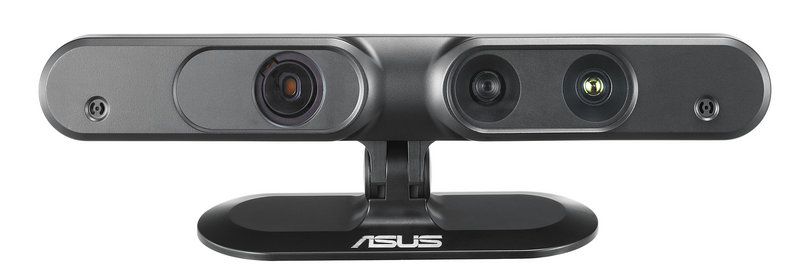
\includegraphics[width=0.4\textwidth]{xtion.jpg}};
    \node [left=0.5cm of asus.north west, yshift=-5mm]{sdfsf};
  \end{tikzpicture}
}

\textbf{Asus Xtion PRO LIVE} \\
\textbf{Distance d'utilisation : }\\
de 0.8 à 3.5 mètres

\textbf{Range de vision : } \\
58\degree Horizontal, 45\degree Vertical, 70\degree Diagonal

\textbf{Resolution : } \\
VGA (640x480) : 30 fps

\textbf{Utilisation intérieur}


\section{Base de données }

\begin{figure}[H]
  \subfloat{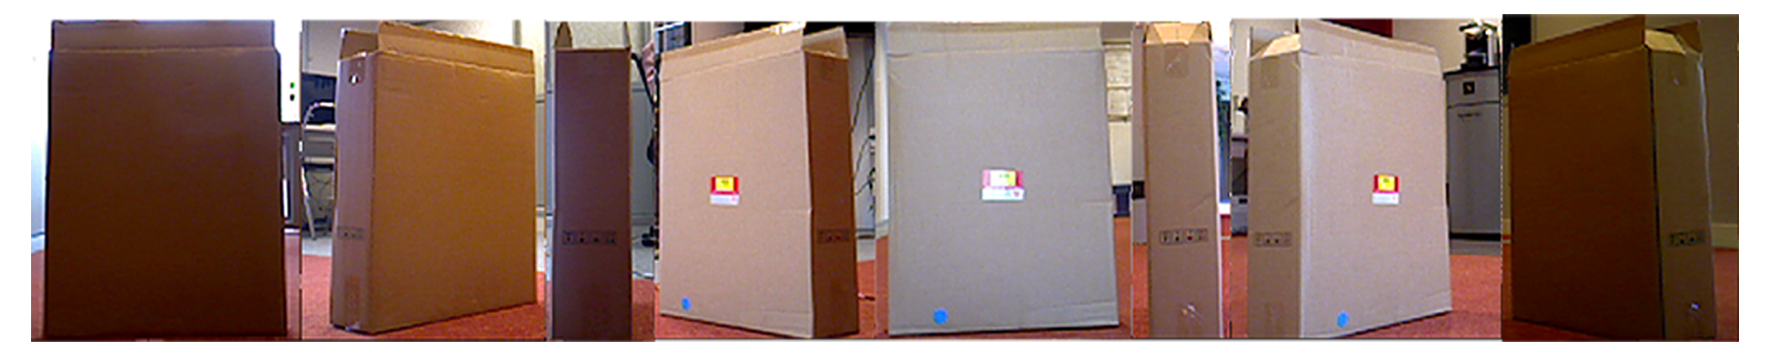
\includegraphics[width=\textwidth]{box_seq.png}}
\end{figure}

\begin{figure}[H]
  \subfloat{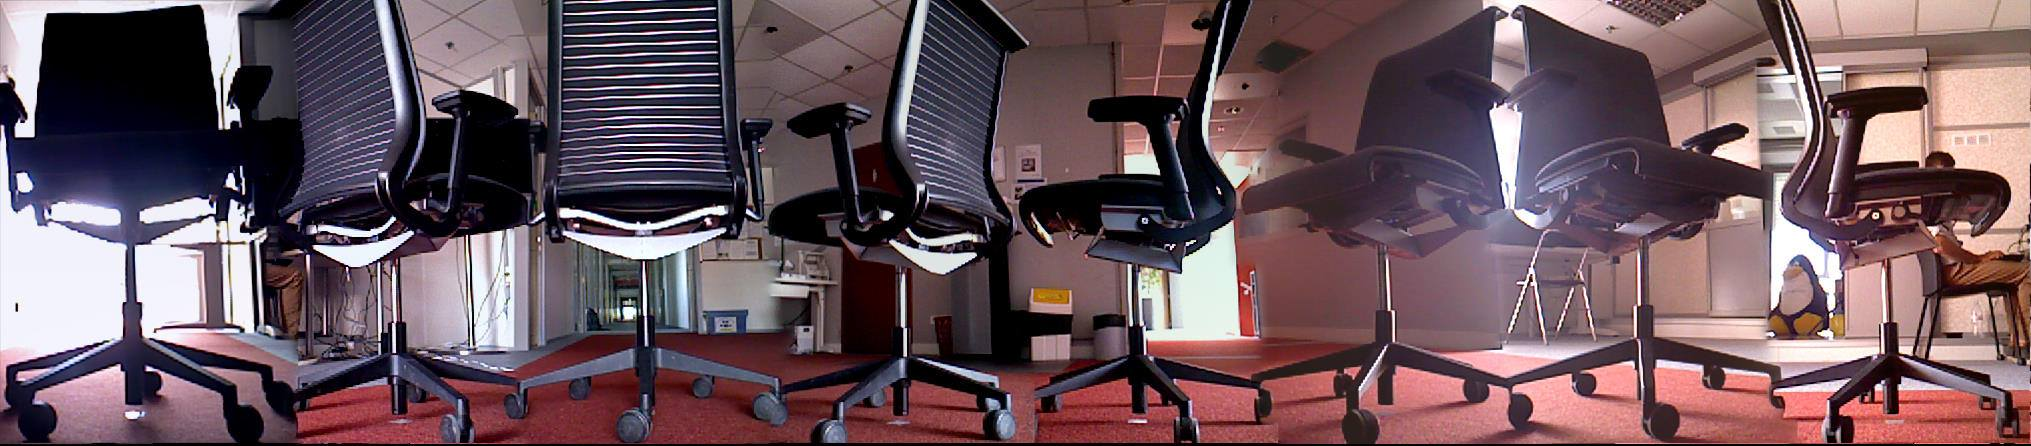
\includegraphics[width=\textwidth]{chair_db.jpg}}
\end{figure}

\begin{figure}[H]
  \subfloat{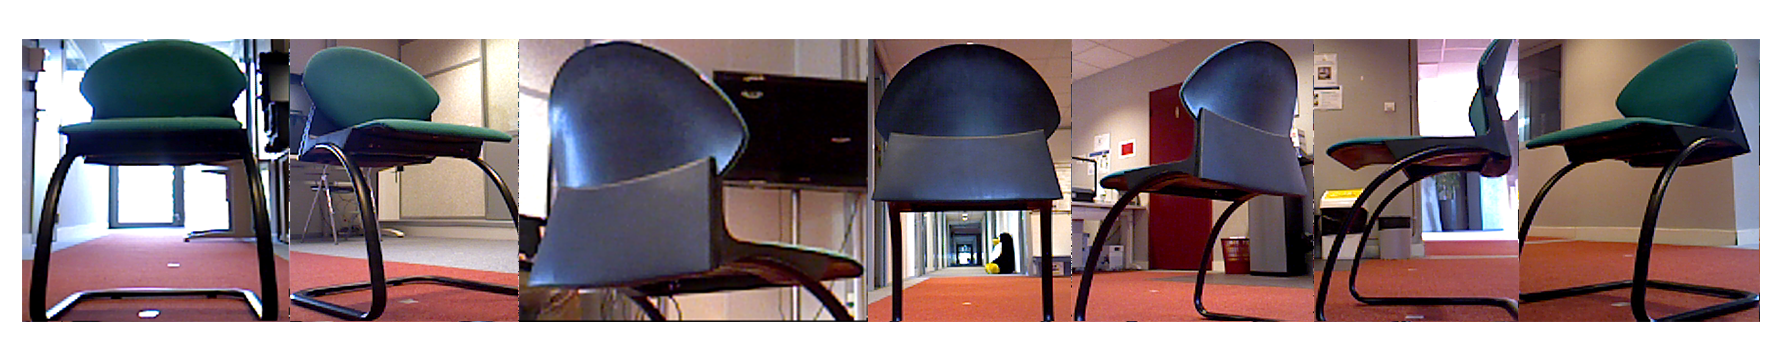
\includegraphics[width=\textwidth]{chair_seq.png}}
\end{figure}

\begin{figure}[H]
  \subfloat{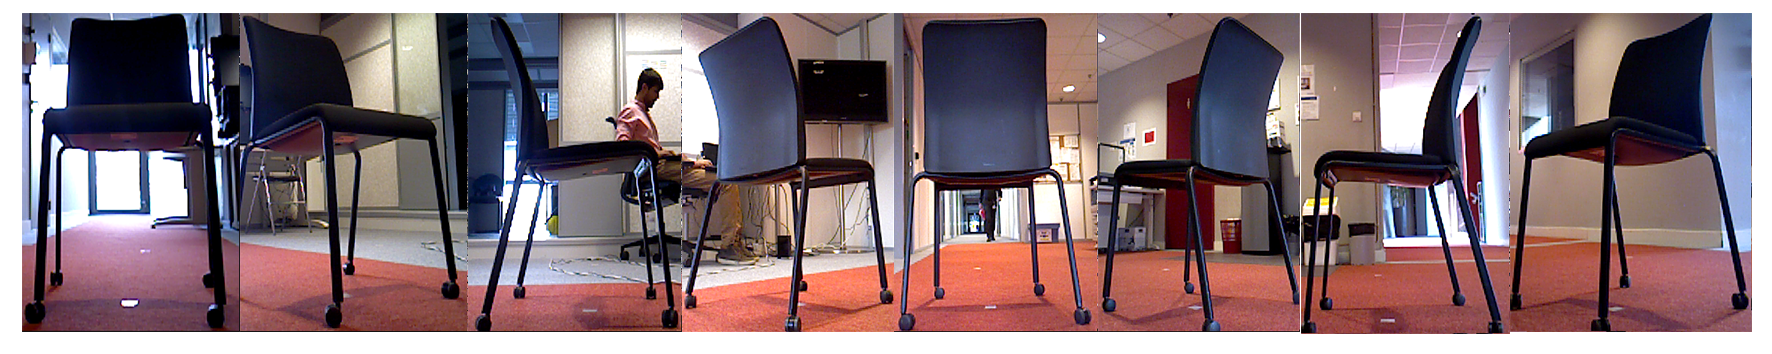
\includegraphics[width=\textwidth]{chair4w.png}}			
\end{figure}


\subsection{Restrictions logiciels}
L' ordinateur embarqué a un puissance de calcul reduit ce que ne permet pas que le node d'acquisition \(openni2\_launch\) tourne correctment. La solution pour l'instant c'était de connecter le capteur Asus sur l'ordinateur portable HP.

\section{ Segmentation }

\subsection{ Paramètres }

\begin{itemize}
\item Distance maximale au capteur : 3 m
\item Distance pour qu'un point soit considéré comme appartenant au plan : 5 cm
\item Taille du \textit{grid} de voxalization : 2 cm
\item Rayon d'estimation de la normale : 2 cm
\item Aire de \textit{smoothing} de la normale : 10 $cm^2$
\item Distance minimal du plan du sol pour qu'il soit considére comme partie de l'objet : 3 cm
\end{itemize}

La plus parts de valeurs étaient choisis telle comme ils était proposé dans la librarie PCL. Quelque autre ont été modifiés pour atteint charactéristique attendue.



\subsection { Floor Detection } 

The major concern goal of the algorithm is to well estimate the floor plan coordinates. From that, other plans like walls could be inferred, supposing they have a fixed geometrical relation. The RANSAC algorithm provide a reasonable solution to the problem and it is already implemented in the PCL library.

Some parameters need to be set, such as deviation from the plan mathematical model.

The parameters used for the robot are described at the annex section.


\subsection{Estimation de la normale}

Pour constituer les informations géométriques l'estimation de la normale du point est d'extrême importance. 

Sont calcul est fait de la manière suivant :
1. Un nombre de voisins est choisi 
2. Ces point *servem* à trouver des paramètres de l'équation du plan tangent et, par consequent, la normale correspondent.

Le méthode adopté pour la bibliothéque PCL correspond à prendre un certain nombre de plus proches voisins définis par un seiul. Un petit seil rendre le calcul faux et un grand prend en compte points distants que peuvent ne pas faire partie du plan estimé.

\url{http://www.pointclouds.org/documentation/tutorials/vfh_recognition.php#vfh-recognition} \\

\url{http://pointclouds.org/documentation/tutorials/fpfh_estimation.php} \\

\url{https://github.com/PointCloudLibrary/pcl/wiki/Overview-and-Comparison-of-Features} \\

\subsection { RANSAC } 

The RANSAC algorithm is a learning method to estimate a given model parameters. Contrary to other estimation algorithms, which considers the whole data represenetative to model estimation, RANSAC suppose the existance of \textbf{inliers or consensus} and \textbf{outliers}  and uses a voting scheme to select between reliable data, that must follow two assumptions: 

\begin{itemize}
\item Noisy data will not vote consistenly for a single model - (few outliners) 
\item Enough good features voting for the same model - (few missing data)
\end{itemize}

\subsubsection{The RANSAC algorithm}

The iterative algorithm is composed of two different stages : 
\begin {itemize}
\item Sample minimal data from dataset requerid to first estimate model parameters.
\item Given a threshold error, it selects data points that are consistent to the model created in the first step.
\end {itemize}

\begin{itemize}
\item Random hypoythetical inliers subset
\item Find model parameters
\item All data tested according to a loss function that determine the \textit{consensus}
\item Finishes when a sufficient number of point belongs to the \textit{consensus}
\end{itemize}

\center \large{\color{blue} If the variables are linear and normally distributed the Bayes filter becomes equal to the Kalman filter.}

%% \caption{My algorithm}\label{euclid}
%% \begin{algorithmic}[1]
%%   \Procedure{RANSAC}{}
%%   \State $\textit{stringlen} \gets \text{length of }\textit{string}$
%%   \State $i \gets \textit{patlen}$
%%   \BState \emph{top}:
%%   \If {$i > \textit{stringlen}$} \Return false
%%   \EndIf
%%   \State $j \gets \textit{patlen}$
%%   \BState \emph{loop}:
%%   \If {$\textit{string}(i) = \textit{path}(j)$}
%%   \State $j \gets j-1$.
%%   \State $i \gets i-1$.
%%   \State \textbf{goto} \emph{loop}.
%%   \State \textbf{close};
%%   \EndIf
%%   \State $i \gets i+\max(\textit{delta}_1(\textit{string}(i)),\textit{delta}_2(j))$.
%%   \State \textbf{goto} \emph{top}.
%%   \EndProcedure
%% \end{algorithmic}
%% \end{algorithm}


\textit{L'Universidad de León } a fait un compte rendu des
\textit{features} implementés sur PCL dans le lien *[8]*. Plus
d'information sur les descripteur et ses implementations sur la
librarie PCL peuvent être retrouvés sur le site
internet \url{http://pointclouds.org}.

Les images sont sauvegardées à l'aide de la librarie OpenCv dans le format 8\_U et .png (Portable Network Graphics).

Les nauges de points sont sauvegardées dans le format .pcd (Point Cloud Data).

Pour sauvegarder les information *provenientes* de la segmentation, les [it]topics de sorti sont souscrit avec rosbag pendent le deplacement du robot. Les messages sauvegardes sont le suivants :

\begin{itemize}
\item v\_objects\_clouds : Vector de nuages de points obtenues pour chaque objet 

\item v\_objects\_image\_and\_mask : Sousimages et mask de chaque objet

\item v\_object\_

\end{itemize}


\section{Planning de Travail}
\begin{itemize}
\item[\checkmark] Mise en place de l'architecture et des protocoles de communication entre composants physiques.
\item[\checkmark] Étude bibliographique initiale pour situer le travail par rapport à l'existant.
\item[\checkmark] Implémentation de l'asservissement d'une caméra PTZ par rapport au retour d'un algorithme de tracking.
\item[\checkmark] Aperçu de certaines limitations de la caméra PTZ qui a été remplacée par une caméra RGB-D.
\item[\checkmark] Utilisation d'un algorithme de segmentation d'objets possibles dans la scène.
\item[\checkmark] Asservissement en boucle ouvert du robot pour la création de la base de données.
\item[\checkmark] Premiers tests pour l'acquisition de la base des données.
\item Résolution des problèmes trouvés lors des premiers tests pour la création de la base de données.
\item Validation de la base de données. Représentativité et reproduction.
\item Étude approfondie de l’état de l'art des modèles et méthodes qui puissent être utiles pour notre problème.
\item Mise en place de la solution et du modèle proposé.
\item Premiers tests et ajustements nécessaires.
\item Mise en œuvre de la solution complète.
\item Validation finale.    
\end{itemize}

\chapter{Le groupe Thales}

\section{Histoire}

Les origines du groupe remontent à 1968 avec la fusion de la Compagnie G\'en\'erale de T\'el\'egraphie sans Fil et des activit\'es d’\'electronique professionnelle de Thomson-Brandt. Cette fusion donne naissance à Thomson-CSF.

Dès 1987, l’entreprise entame une restructuration en profondeur de ses activit\'es et met en place une strat\'egie d’expansion vers l’Europe.

En 1998, le gouvernement français cède une partie de ses actions aux soci\'et\'es Aerospatiale, Alcatel et Dassault. Le groupe bascule alors dans le secteur priv\'e, cela entraîne aussi une expansion des activit\'es, notamment dans le secteur de la d\'efense, au-delà de l’Europe, comme en Australie, en Cor\'ee ou à Singapour. Les activit\'es se sont aussi diversifi\'ees et s’articulent principalement autour de la d\'efense, l’a\'eronautique et les technologies de l’information.

En 2000, Thomson-CSF devient Thales. Le groupe devient un leader dans les domaines de la d\'efense et de l’a\'eronautique et renforce sa pr\'esence dans le domaine de la s\'ecurit\'e civile.

En 2009, Dassault devient l’actionnaire majoritaire du groupe en rachetant les parts d’Alcatel. De ce fait, en 2010 l’organisation de Thales est modifi\'ee suivant un système bas\'e sur 3 zones g\'eographiques et 7 divisions afin de simplifier son fonctionnement et am\'eliorer ses performances.

\section{Secteurs d’activit\'e}

Thales est un groupe d’\'electronique sp\'ecialis\'e dans l’a\'erospatial, la d\'efense et les technologies de l’information. Cot\'e à la bourse de Paris, pr\'esent dans 56 pays et employant 66 500 collaborateurs, Thales est un des leaders mondiaux des systèmes d’information critiques sur les march\'es de l’a\'eronautique et de l’espace, de la d\'efense et de la s\'ecurit\'e. Avec environ 14,2 milliards d’euros de chiffre d’affaire en 2013, le capital du groupe est d\'etenu à 27\% par l’État français, 26\% par Dassault Aviation et les 47\% restants sont flottants. Le portefeuille du groupe est \'equilibr\'e avec 55\% de commandes d\'edi\'ees à la D\'efense et 40\% au Civil. L’innovation constitue un secteur important pour Thales. Aujourd’hui elle d\'epasse le seul cadre technologique pour irriguer tous les champs de l’entreprise, de la recherche et d\'eveloppement à l’activit\'e commerciale.  Les d\'epenses de recherche et d\'eveloppement repr\'esentent 20\% de l'activit\'e du groupe. Avec plus de 25 000 chercheurs et ing\'enieurs, un portefeuille regroupant 15000 brevets et plus de 30 accords de coop\'eration avec des universit\'es et des laboratoires publics en Europe, aux États-Unis et en Asie, Thales occupe une place de r\'ef\'erence dans les domaines de la haute technologie et de l’innovation.

Les travaux de recherche amont sont essentiellement conduits au sein de Thales Research \& Technology (TRT), centre de recherche du groupe Thales en France, qui regroupe environ 500 experts autour de trois domaines techniques cl\'es :

\begin{itemize}
  \item Électronique, \'electromagn\'etisme et optronique
  \item Logiciel et système d’information
  \item Sciences de l’information et de la cognition
\end{itemize}
  
Et dont les activit\'es s’opèrent au sein de sept laboratoires :

\begin{itemize}
  \item Ing\'enierie des systèmes logiciels
  \item Analyse des sources d’information
  \item S\'ecurit\'e sur Internet
  \item Recherche en infra-rouge et imagerie polarim\'etrique
  \item Dualit\'e et technologies de souverainet\'e
  \item S\'ecurit\'e biologique et chimique
  \item Nano-magn\'etisme
\end{itemize}

Les liens tiss\'es entre ces \'equipes de recherche et les communaut\'es acad\'emique, scientifique et industrielle, se mettent en place grâce à l’implantation des laboratoires de TRT dans des campus universitaires. En France, c’est le cas du site de Palaiseau qui est implant\'e sur le campus de l’Ecole Polytechnique.

\section{Organisation}

Le groupe Thales est organis\'e de façon matricielle : par pays et par domaine d’activit\'e regroupant ainsi six divisions repr\'esent\'ees dans l’organigramme ci-dessous . Le laboratoire ThereSIS, dans le lequel s’est d\'eroul\'e le stage est aussi mis en \'evidence

%(figure \ref{fig:organigramme})

% TODO Organigramme
% \begin{figure}[!htb]
%   \centering
%   \includegraphics[width=10cm]{temp}
%   \caption{L’organigramme de Thales}
%   \label{fig:organigramme}
% \end{figure}

\section{Pr\'esentation de ThereSIS}

\paragraph{} Au sein de la branche « Systèmes d’information et de Communications S\'ecuris\'es », se trouve la filiale Thales Service SAS qui travaille sur la conception, le d\'eveloppement et l’int\'egration des systèmes d’information critiques pour les entreprises et les gouvernements.

\paragraph{} C’est à l’int\'erieur même de Thales Service SAS que se trouve le laboratoire d’innovation ThereSIS (Thales European Research centre for Security \& Information Systems). Ce laboratoire est n\'e en Septembre 2006 d’une volont\'e de renforcer le leadership de Thales dans le domaine particulier de l’ICT vis-à-vis notamment de la communaut\'e europ\'eenne. Ce laboratoire de recherches appliqu\'ees est l’un des quatre laboratoires de GBU SIX, d\'edi\'es aux Etudes Amont, avec TAI (Technologie Avanc\'ees de l’Information), SC2 (Software Core) et le CENTAI (Centre d’Excellence Nouvelles Techniques Analyse de l’Information). Un des objectifs communs est de d\'evelopper des diff\'erenciateurs techniques au b\'en\'efice des unit\'es op\'erationnelles de la GBU et plus largement du groupe Thales.  L’\'equipe initiale \'etait compos\'ee de 20 experts en système de s\'ecurit\'e d’information critique. Ensuite, le concept fut \'etendu au domaine de la "S\'ecurit\'e Physique" en 2007, et le laboratoire a vu son effectif s’\'elever à 45 employ\'es. Aujourd’hui l’\'equipe de ThereSIS compte environ 70 personnes.

\section{Secteurs d’activit\'e}

\paragraph{} Install\'e à Palaiseau, dans les locaux de TRT, ThereSIS d\'eveloppe des solutions innovantes dans le domaine de la s\'ecurit\'e et de la protection des infrastructures critiques, telles que les a\'eroports, les centrales nucl\'eaires, les gares, etc. Ces activit\'es se concentrent aujourd’hui sur les sujets suivants :

\begin{itemize}
  \item La s\'ecurit\'e physique avec le d\'eveloppement de systèmes a base de capteurs innovants, le traitement intelligent de la vid\'eo, la gestion de crise et l’interop\'erabilit\'e des systèmes.
  \item Les m\'ecanismes et les services de s\'ecurit\'e de système d’information et le management d’identit\'es.
  \item La supervision de la cyber-s\'ecurit\'e des architectures critiques et l’aide à la d\'ecision adaptable aux contextes m\'etiers.
  \item Les modèles, outils et services de s\'ecurit\'e et de management de la multi-conformit\'e en dynamique pour les architectures de type SOA.
  \item La s\'ecurisation et la supervision des architectures de service vitalis\'ees et le "cloud computing"
  \item Les interfaces multimodales et les dialogues hommes-machines.
  \item La mod\'elisation directement ex\'ecutable de processus complexes, leur interface graphique et leur s\'emantique.
  \item Les environnements synth\'etiques et leurs apports pour les systèmes d’information critique avec la simulation des comportements humains.
\end{itemize}

\section{Le laboratoire Video Technologies \& New Sensors}

\paragraph{} Le laboratoire Video Technologies \& New Sensors est compos\'e de deux domaines : l'analyse vid\'eo et les syst\`emes de perception. L'analyse vid\'eo traite en particulier du d\'eveloppent d'algorithmes avanc\'es de traitement d'image via un laboratoire commun entre Thales et le CEA\footnote{Commissariat \`a l'\'Energie Atomique et aux \'Energies Alternatives.}, baptis\'e VisionLab.

% \appendix
% \chapter{Implantation du Système Étendu}


	Différemment de l'implantation du système de Paillier, l'implantation du système étendu a été faite seulement en \verb!Python!.
	Comme dit dans la page \pageref{chap:implantation}, dans \verb!Python! le traitement des grand entiers est intégré et permet 
	le dé\-ve\-lop\-pe\-ment plus concerné avec l'algorithme qu'avec les particularités des structures et représentations.


	Dans l'extension, grâce à la utilisation de la base fixe $n+1$, on a diverses optimisations qui peuvent être mises en œuvre, comme
	par exemple le calcul de $(1+n)^m\mod{n^{s+1}}$ qui peut être développé $1+mn+\frac{m(m-1)}{2}n^2+\dots+n^s\binom{m}{s}\mod{n^{s+1}}$, 
	cette optimisation est implantée par la méthode ~\verb!powGOpt!. Une table des fonctions disponibles se trouve dans la page \pageref{syset:listef}.


	L'utilisation du logiciel de profil \verb!cProfile! permet de trouver le goulet d'étranglement, qui ne diffère pas de l'implantation
	précédente, à savoir: la méthode \verb!pow!.


	\begin{lstlisting}[language=python,caption=Fonction de chiffrement du système étendu en Python, label=code:chiffet]	
	def encrypt(self,m,pubKey,r = None,s=None):
		if r == None:
			r = randomPhi(pubKey.n);
		if s == None:
			s = self.upper_boundNCache(pubKey.n,m);
		if 2*s*s > pubKey.n:
			raise Exception("Impossible to encrypt, the block is too large");
		potnn = self.getCachePot('n',pubKey.n,s+1);
		potn  = self.getCachePot('n',pubKey.n,s);
		return (self.powGOpt(pubKey.n,m,s)*pow(r,potn,potnn))%potnn;
	
	def decrypt(self,c,pvtKey,s=None):
		if s == None:
			s = self.upper_boundNCache(pvtKey.n,c);
			s-=1;	
		if 2*s*s > pvtKey.n:
			raise Exception("Impossible to decrypt, the block is too large");
		if not self.optimizeCRT:
			potnn = self.getCachePot('n',pvtKey.n,s+1);
			potn  = self.getCachePot('n',pvtKey.n,s  );
			d=pvtKey.lam*number.inverse(pvtKey.lam,potn); 
			pjid = pow(c ,d,potnn);
			jid  = self.findI(pjid,'n',pvtKey.n,'n',pvtKey.n,s);
			return jid;
		potpp = self.getCachePot('p',pvtKey.p,s+1);
		potqq = self.getCachePot('q',pvtKey.q,s+1);
		potp  = self.getCachePot('p',pvtKey.p,s);
		potq  = self.getCachePot('q',pvtKey.q,s);
		potn  = self.getCachePot('n',pvtKey.n,s);
		cp = c%potpp;
		cq = c%potqq;
		cp = pow(cp,pvtKey.p-1,potpp);
		cq = pow(cq,pvtKey.q-1,potqq);
		ppjid = self.findI(cp,'n',pvtKey.n,'p',pvtKey.p,s,q=pvtKey.q);
		qqjid = self.findI(cq,'n',pvtKey.n,'q',pvtKey.q,s,q=pvtKey.p);
		ppjid*=number.inverse(pvtKey.p-1,potp);
		qqjid*=number.inverse(pvtKey.q-1,potq);
		return CRT(ppjid,qqjid,potp,potq)%(potn)
	\end{lstlisting}


	\section{Liste de fonctions Implantées}
	\label{syset:listef}
	
	Les classes qui gardent les informations sur les clés publiques et privées en \verb!Python!:
	\begin{lstlisting}[language=python,caption=Structures des Clés en Python, label=code:structgen]
dir(GenPaillierPvtKey()): ['__doc__', '__init__', '__module__', '__str__', 'lam', 'n', 'p', 'q']
dir(GenPaillierPubKey(pvt)): ['__doc__', '__init__', '__module__', '__str__', 'n']
	\end{lstlisting}

Les fonctions mises en œuvre avec la langage \verb!python!:

	\begin{itemize} \renewcommand{\labelitemi}{} \renewcommand{\labelitemii}{$~~argument$}

		\item \textbf{GenPaillier}:Constructeur.
			\begin{itemize}
				\item \verb!cachepowN = True!:Si \verb!True!, active 
				le cache de puissances de $n$. Par défaut \verb!True!.
				\item \verb!cachefact= True!:Si \verb!True!, active 
				le cache des factoriels. Par défaut \verb!True!.
				\item \verb!optimizeg = True!: Si \verb!True!, optimise  
				l'exponentiation de $n+1$ dans le chiffrement.
				\item \verb!optimizeCRT = True!: Si \verb!True!, optimise  
				avec le Théo\-rè\-me du Reste Chinois.
			\end{itemize}
		\item \textbf{powGOpt}: Mètre en œuvre l'optimisation dans le développent de $(1+n)^{po} \mod{n^{s+1}}$.
			\begin{itemize}
				\item \verb!n!: Entière, la valeur $n$ dans $(1+n)^{po}$.
				\item \verb!po!: Entière, la valeur $po$.
				\item \verb!s!: Entière, la valeur $s$.
			\end{itemize}
		\item \textbf{getCachePot}: Retourne une puissance en cache et si nécessaire, calcule.
			\begin{itemize}
				\item \verb!name!: Nom de la valeur. Ex.:\verb!'n'! 
				\item \verb!val!: Valeur de la base.
				\item \verb!s!: Exposant.
			\end{itemize}
		\item \textbf{getFactNSCache}: Retourne les valeurs mémorisées (programmation dynamique) de factoriel de $n$ modulo $nbase^s$.
			\begin{itemize}
				\item \verb!n!: Entière $n$.
				\item \verb!basename!: Nom de la base (en cache). Ex.:\verb!'nbase'! 
				\item \verb!nbase!:Entière $nbase$.
				\item \verb!s!: Entière $s$.
			\end{itemize}
		\item \textbf{upper\_boundNCache}: Retourne la valeur estimée pour $s$ dans le chiffrement  de 
		$m$ depuis la valeur chiffré $value$. C'est-à-dire, le plus petit $s$ tel que $value \in \Mgr{Z}{n^{s+1}}$.
			\begin{itemize}
				\item \verb!n!: La base (clé publique).
				\item \verb!value!: La valeur chiffrée.
			\end{itemize}
		\item \textbf{findI}: Implante l'algorithme de logarithme modulaire vu dans le Chapitre \ref{chap:jurik}.
			\begin{itemize}
				\item \verb!a!: La puissance de $1+n$ dans l'anneau $\Mgr{Z}{n^{s}}$.
				\item \verb!namen!: Le nom de \verb!n! pour le cache.
				\item \verb!n!:  L'entier $n$ de la clé publique.
				\item \verb!namep!: Le nom de \verb!p! pour le cache (voir en bas).
				\item \verb!p!: L'entier à être utilisé par la fonction $L$
				\item \verb!s!: La valeur estimé par \verb!findI!. Il est recommandé l'utilisation de la fonction \verb!findI!, par contre si le protocole force $s$ il n'est pas nécessaire.
				\item \verb!q=1!: $n/p$, par défaut $1$.
			\end{itemize}
		\item \textbf{encrypt}: Chiffre le message $m$.
			\begin{itemize}
				\item \verb!m!: Un entier, le message à être chiffré.
				\item \verb!pubKey!: La clé publique.
				\item \verb!r = None!: La valeur aléatoire qui 
				sera ajoutée au chiffrement. Si \verb!None!, 
				la va\-leur est prise aléatoirement avec
				la fonction par défaut de la bibliothèque
				\verb!PyCrypto!.
				\item \verb!s=None!: La valeur de $s$ qui 
				doit être utilisé. Si $s$ est trop petit, 
				la fonction jette l'exception 	{\em Impossible 
				to encrypt, the block is too large}. Si \verb!None!, 
				la valeur est trouvé avec le méthode \verb!upper\_boundNCache!
			\end{itemize}
	
		\item \textbf{decrypt}: La fonction de déchiffrement.
			\begin{itemize}
				\item \verb!c!: La valeur à être déchiffrée.
				\item \verb!pvtKey!: La clé privé.
				\item \verb!s=None!: Le paramètre $s$ de déchiffrement. Si \verb!None! il est estimé depuis la taille en bits de $c$.
			\end{itemize}
	\end{itemize}


%	\begin{itemize} \renewcommand{\labelitemi}{} \renewcommand{\labelitemii}{$~~argument$}
%		\item \textbf{GenPaillier}: Constructeur.
%			\begin{itemize}
%				\item \verb!cachepowN!: Si \verb!True!, active 
%				le cache de puissances de $n$. Par défaut \verb!True!.
%				\item \verb!cachefact!: Si \verb!True!, active 
%				le cache des factoriels. Par défaut \verb!True!.
%				\item \verb!optimizeg!: Si \verb!True!, optimise  
%				l'exponentiation de $n+1$ dans le chiffrement.
%				Par défaut \verb!True!.
%			\end{itemize}
%			%self,cachepowN = True,cachefact= True,optimizeg = True}
%		\item \textbf{powGOpt}: Mètre en œuvre l'optimisation dans le développent de $(1+n)^{po} \mod{n^{s+1}}$.
%			\begin{itemize}
%				\item \verb!n!: Entière, la valeur $n$ dans $(1+n)^{po}$.
%				\item \verb!po!: Entière, la valeur $po$.
%				\item \verb!s!: Entière, la valeur $s$.
%			\end{itemize}
%
%		\item \textbf{getFactNSCache}: Retourne les valeurs mémorisées (programmation dynamique) de factoriel de $n$ modulo $nbase^s$. 
%			\begin{itemize}
%				\item \verb!n!: Entière $n$.
%				\item \verb!nbase!: Entière $nbase$.
%				\item \verb!s!: Entière $s$.
%			\end{itemize}
%
%		\item \textbf{getPowNCache}: Retourne les valeurs mémorisées de $n^{powv}$
%			\begin{itemize}
%				\item \verb!n!: Entière $n$
%				\item \verb!powv!: Entière $powv$
%			\end{itemize}
%		\item \textbf{upper\_boundNCache}: Retourne la valeur estimé pour $s$ dans la chiffrage de $m$ depuis la valeur chiffré $value$. C'est-à-dire, le plus petit $s$ tel que $value \in \Mgr{Z}{n^{s+1}}$.
%			\begin{itemize}
%				\item \verb!n!: La base (clé publique).
%				\item \verb!value!: La valeur chiffré.
%			\end{itemize}
%		\item \textbf{findI}: Implante le algorithme de logarithme modulaire vu dans le Chapitre \ref{chap:jurik}.
%			\begin{itemize}
%				\item \verb!a!: La puissance de $1+n$ dans l'anneau $\Mgr{Z}{n^{s}}$.
%				\item \verb!n!: Le entière $n$ de la clé publique.
%				\item \verb!s!: La valeur estimé par \verb!findI!. Il est recommandé la utilisation de la fonction \verb!findI!, par contre si le protocole force $s$ il n'est pas nécessaire.
%			\end{itemize}
%		\item \textbf{encrypt}: Chiffre le message $m$.
%			\begin{itemize}
%				\item \verb!m!: Un entière, le message à être chiffré.
%				\item \verb!pubKey!: La clé publique.
%				\item \verb!r = None!: La valeur aléatoire qui 
%				sera ajouté au chiffrement. Si \verb!None!, 
%				la va\-leur est prise aléatoirement avec
%				la fonction par défaut de la bibliothèque
%				\verb!PyCrypto!.
% 
%				\item \verb!s = None!: La valeur de $s$ qui 
%				doit être utilisé. Si $s$ est trop petit, 
%				la fonction jette la exception 	{\em Impossible 
%				to encrypt, the block is too large}. Si \verb!None!, 
%				la valeur est trouvé avec le méthode \verb!upper\_boundNCache!
%			\end{itemize}
%		\item \textbf{decrypt}: La fonction de déchiffrement.
%			\begin{itemize}
%				\item \verb!c!: La valeur à être déchiffré.
%				\item \verb!pvtKey!: La clé privé.
%				\item \verb!s = None!: Le paramètre $s$ de déchiffrage. Si \verb!None! il est estimé depuis la taille en bits de $c$.
%			\end{itemize}
%
%%	def powGOpt(self,n,po,s):
%%	def getFactNSCache(self,n,nbase,s):
%%	def getPowNCache(self,n,powv):
%%	def upper_boundNCache(self,n,value):
%%	def findI(self,a,n,s):
%%	def encrypt(self,m,pubKey,r = None,s=None):
%%	def decrypt(self,c,pvtKey,s=None):
%	\end{itemize}

	\section{Génération des clés}

	La génération des clés suit la méthode du système de Paillier.

	\section{Benchmark}

L'optimisation par l'application du Théorème du Reste Chinois est surprenant,
elle rends le déchiffrement plus rapide avec la augmentation de la taille de $n$ et la valeur de $s$, en attendant 
 $14.78$ fois plus rapide par rapport à l'instance sans le TRC quand $s = 3$ et $|n| = 2048$. 
 Dans le déchiffrement, l'optimisation de l'exponentiation de $n+1$ avec le développent de Newton rends le code plus rapide 
 avec un facteur de $1.88$ quand $s=3$ et $|n|=2048$.

Processeur: \verb!Intel(R) Core(TM)2 Duo CPU E6550  @ 2.33GHz!

Système d'exploitation:\hfill \verb!Linux version 3.3.5-2.fc16.x86_64!

	\hfill		\verb!(mockbuild@x86-04.phx2.fedoraproject.org)!

	\hfill		\verb!(gcc version 4.6.3 20120306 (Red Hat 4.6.3-2) (GCC))!

	\hfill		\verb!#1 SMP Tue May 8 11:24:50 UTC 2012i!

Version de \verb!Python!: \verb!Python 2.7.3!

Version de \verb!GMP!: \verb!libgmp.so.3.5.2!


\begin{table}[hlc]
\center
\caption{Temps du programme en secondes avec $|n|$ = 1024/2048 bits pour 300 appels.}
\begin{tabular}{|c |c|c|c|c| |c | c|c|}
\hline
%\hline
%$\multirow{2}{*}{$|n|$}$&\multicolumn{4}{|c|}{C}\\
%		\cline{2-5}
%                    &gen&chiff&dechiff&TRC\\
%\hline
\begin{sideways}s\end{sideways}&%
\begin{sideways}Cache dans $n^i$\end{sideways}&%
\begin{sideways}Cache du Factoriel\end{sideways}&%
\begin{sideways}Optimisation de $(n+1)^i$\end{sideways}&%
\begin{sideways}Reste Chinois\end{sideways}&%
%\begin{sideways}$|n|$\end{sideways}&%
\begin{sideways}G\'en\'eration des cl\'es\end{sideways}&%
\begin{sideways}Chiffrement\end{sideways}&%
\begin{sideways}D\'echiffrement\end{sideways}\\%
\hline
\hline
1 & N& N& N& N & 13.88 / 61.48 & 21.72 / 147.8 & 33.7 / 223.76 \\
1 & N& N& N& O & 14.37 / 62.97 & 22.43 / 155.47 & 5.14 / 25.72 \\
1 & N& N& O& N & 13.99 / 63.07 & 14.92 / 107.59 & 31.54 / 217.81 \\
1 & N& O& N& N & 14.07 / 65.48 & 22.58 / 143.16 & 33.87 / 224.18 \\
1 & O& N& N& N & 14.31 / 61.68 & 23.08 / 149.68 & 31.01 / 227.2 \\
1 & O& O& O& O & 13.95 / 60.28 & 15.95 / 113.09 & 5.46 / 29.05 \\
\hline
\hline
2 & N& N& N& N & 14.51 / 60.51 & 97.7 / 645.38 & 88.58 / 617.4 \\
2 & N& N& N& O & 14.36 / 58.84 & 96.97 / 680.33 & 9.08 / 58.65 \\
2 & N& N& O& N & 13.2 / 61.82 & 59.98 / 403.15 & 87.46 / 625.18 \\
2 & N& O& N& N & 13.53 / 62.35 & 96.5 / 650.89 & 90.39 / 624.16 \\
2 & O& N& N& N & 14.49 / 59.65 & 95.03 / 672.41 & 87.88 / 612.15 \\
2 & O& O& O& O & 13.36 / 62.93 & 57.43 / 402.16 & 9.94 / 50.18 \\
\hline
\hline
3 & N& N& N& N & 13.93 / 61.13 & 236.46 / 1671.15 & 178.9 / 1242.47 \\
3 & N& N& N& O & 13.66 / 63.88 & 238.38 / 1598.63 & 14.88 / 85.71 \\
3 & N& N& O& N & 13.75 / 61.51 & 125.63 / 937.21 & 177.32 / 1265.05 \\
3 & N& O& N& N & 13.42 / 58.82 & 238.36 / 1642.77 & 182.26 / 1250.68 \\
3 & O& N& N& N & 13.42 / 63.97 & 227.38 / 1651.81 & 174.48 / 1236.89 \\
3 & O& O& O& O & 13.99 / 62.99 & 126.34 / 939.06 & 14.62 / 84.35 \\
\hline
\end{tabular}
\end{table}




	

% \chapter{Profils}
\begin{figure}[hlc]
	\center

	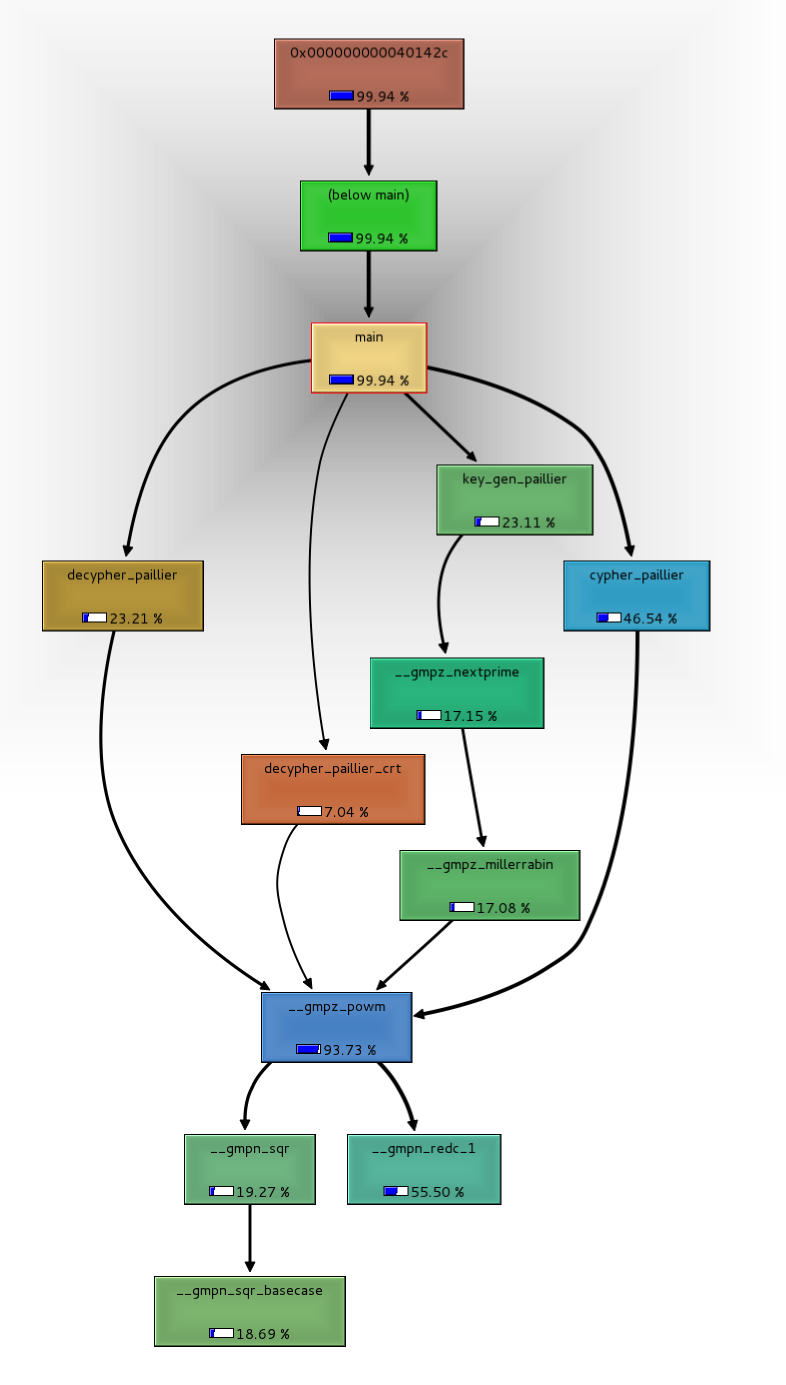
\includegraphics[height=0.8\textheight]{proff.eps}
	
	\caption{Profil montrant l'utilisation des ressources par les différentes méthodes implantées.} 
\end{figure}

Le profil a été réalisé sur le code suivant:
\begin{lstlisting}[language=C,emph={},caption=Code du test de profil., label=code:profil]
#include <stdio.h>
#include "paillier.h"
int main(){
	pvt_key pvt;
	public_key pub;
	mpz_t message, encripted, message_prime, tmp;
	int i;
	_rnd_paillier= NULL;

	mpz_init(message);
	mpz_init(message_prime);
	mpz_init(encripted);
	mpz_init(tmp);

	pvt = key_gen_paillier(1024LU);
	pub = get_public_paillier(pvt);

	for(i = 0;i<10;i++){
		checkRandomInit();
		mpz_urandomm(message, *_rnd_paillier, pub->n);
		cypher_paillier(encripted,message,pub);
		decypher_paillier(message_prime,encripted,pvt);
		decypher_paillier_crt(message_prime,tmp,encripted,pvt);
	}
	cleankeys(&pvt,NULL);
	cleankeys(NULL,&pub);
	return 0;
}
\end{lstlisting}

% \chapter{Implantation en C}
\label{Impl:C}
%\lstinputlisting[language=C,emph={}]{../src/paillier.c}
\chapter{Implantation en Python}
\label{Impl:Py}
%\lstinputlisting[language=Python]{../python/paillier.py}
\chapter{Profils}
\begin{figure}[hlc]
\center
%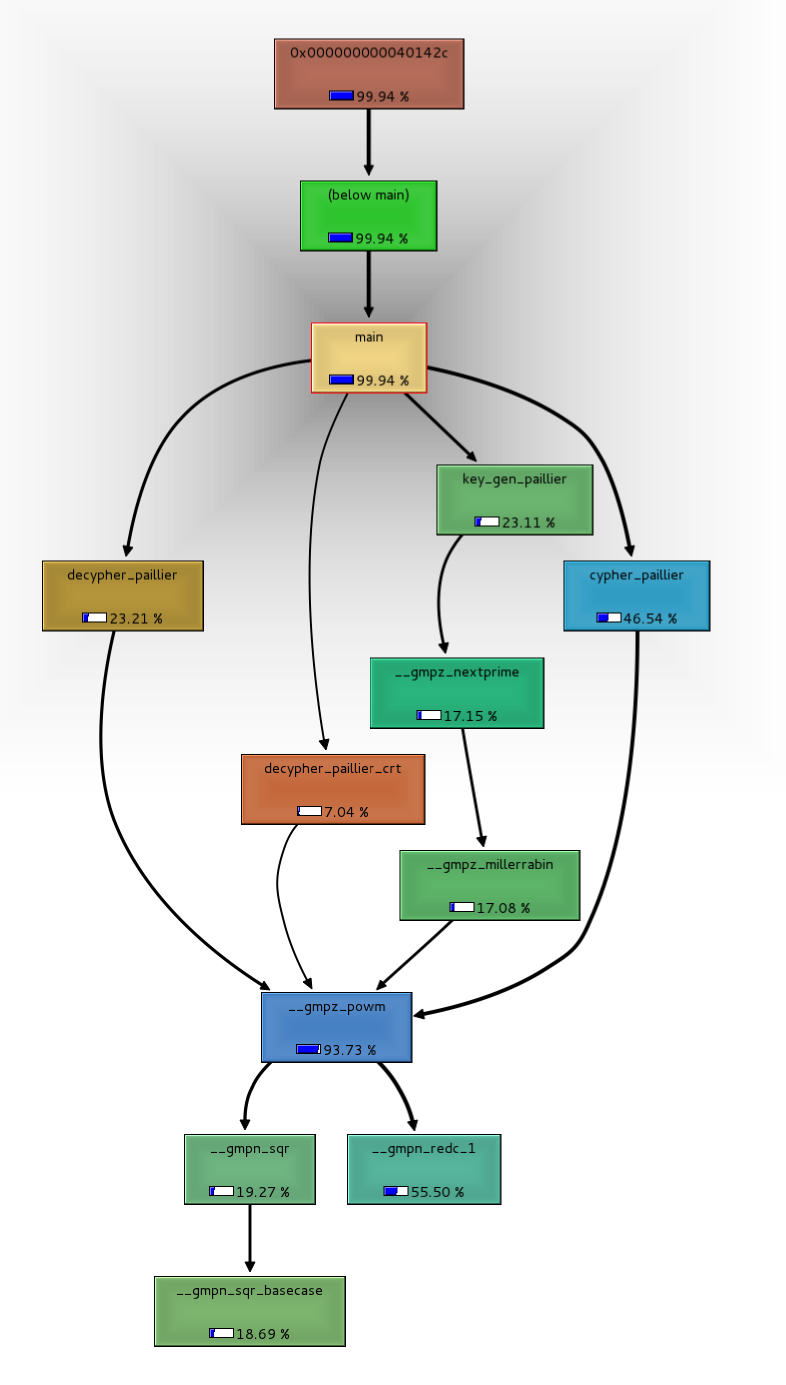
\includegraphics[height=0.6\textheight]{proff.eps}
\end{figure}


\end{document}



